\documentclass[twoside]{book}

% Packages required by doxygen
\usepackage{calc}
\usepackage{doxygen}
\usepackage{graphicx}
\usepackage[utf8]{inputenc}
\usepackage{makeidx}
\usepackage{multicol}
\usepackage{multirow}
\usepackage{textcomp}
\usepackage[table]{xcolor}

% Font selection
\usepackage[T1]{fontenc}
\usepackage{mathptmx}
\usepackage[scaled=.90]{helvet}
\usepackage{courier}
\usepackage{amssymb}
\usepackage{sectsty}
\renewcommand{\familydefault}{\sfdefault}
\allsectionsfont{%
  \fontseries{bc}\selectfont%
  \color{darkgray}%
}
\renewcommand{\DoxyLabelFont}{%
  \fontseries{bc}\selectfont%
  \color{darkgray}%
}

% Page & text layout
\usepackage{geometry}
\geometry{%
  a4paper,%
  top=2.5cm,%
  bottom=2.5cm,%
  left=2.5cm,%
  right=2.5cm%
}
\tolerance=750
\hfuzz=15pt
\hbadness=750
\setlength{\emergencystretch}{15pt}
\setlength{\parindent}{0cm}
\setlength{\parskip}{0.2cm}
\makeatletter
\renewcommand{\paragraph}{%
  \@startsection{paragraph}{4}{0ex}{-1.0ex}{1.0ex}{%
    \normalfont\normalsize\bfseries\SS@parafont%
  }%
}
\renewcommand{\subparagraph}{%
  \@startsection{subparagraph}{5}{0ex}{-1.0ex}{1.0ex}{%
    \normalfont\normalsize\bfseries\SS@subparafont%
  }%
}
\makeatother

% Headers & footers
\usepackage{fancyhdr}
\pagestyle{fancyplain}
\fancyhead[LE]{\fancyplain{}{\bfseries\thepage}}
\fancyhead[CE]{\fancyplain{}{}}
\fancyhead[RE]{\fancyplain{}{\bfseries\leftmark}}
\fancyhead[LO]{\fancyplain{}{\bfseries\rightmark}}
\fancyhead[CO]{\fancyplain{}{}}
\fancyhead[RO]{\fancyplain{}{\bfseries\thepage}}
\fancyfoot[LE]{\fancyplain{}{}}
\fancyfoot[CE]{\fancyplain{}{}}
\fancyfoot[RE]{\fancyplain{}{\bfseries\scriptsize Generated on Thu Nov 6 2014 12\-:22\-:30 for libmae by Doxygen }}
\fancyfoot[LO]{\fancyplain{}{\bfseries\scriptsize Generated on Thu Nov 6 2014 12\-:22\-:30 for libmae by Doxygen }}
\fancyfoot[CO]{\fancyplain{}{}}
\fancyfoot[RO]{\fancyplain{}{}}
\renewcommand{\footrulewidth}{0.4pt}
\renewcommand{\chaptermark}[1]{%
  \markboth{#1}{}%
}
\renewcommand{\sectionmark}[1]{%
  \markright{\thesection\ #1}%
}

% Indices & bibliography
\usepackage{natbib}
\usepackage[titles]{tocloft}
\setcounter{tocdepth}{3}
\setcounter{secnumdepth}{5}
\makeindex

% Hyperlinks (required, but should be loaded last)
\usepackage{ifpdf}
\ifpdf
  \usepackage[pdftex,pagebackref=true]{hyperref}
\else
  \usepackage[ps2pdf,pagebackref=true]{hyperref}
\fi
\hypersetup{%
  colorlinks=true,%
  linkcolor=blue,%
  citecolor=blue,%
  unicode%
}

% Custom commands
\newcommand{\clearemptydoublepage}{%
  \newpage{\pagestyle{empty}\cleardoublepage}%
}


%===== C O N T E N T S =====

\begin{document}

% Titlepage & ToC
\hypersetup{pageanchor=false}
\pagenumbering{roman}
\begin{titlepage}
\vspace*{7cm}
\begin{center}%
{\Large libmae }\\
\vspace*{1cm}
{\large Generated by Doxygen 1.8.6}\\
\vspace*{0.5cm}
{\small Thu Nov 6 2014 12:22:30}\\
\end{center}
\end{titlepage}
\clearemptydoublepage
\tableofcontents
\clearemptydoublepage
\pagenumbering{arabic}
\hypersetup{pageanchor=true}

%--- Begin generated contents ---
\chapter{Hierarchical Index}
\section{Class Hierarchy}
This inheritance list is sorted roughly, but not completely, alphabetically\-:\begin{DoxyCompactList}
\item \contentsline{section}{mae\-:\-:fl\-:\-:angular\-\_\-joint}{\pageref{classmae_1_1fl_1_1angular__joint}}{}
\item \contentsline{section}{mae\-:\-:fl\-:\-:angular\-\_\-skeleton}{\pageref{classmae_1_1fl_1_1angular__skeleton}}{}
\item \contentsline{section}{mae\-:\-:math\-:\-:basis}{\pageref{classmae_1_1math_1_1basis}}{}
\item \contentsline{section}{mae\-:\-:bone}{\pageref{classmae_1_1bone}}{}
\item \contentsline{section}{mae\-:\-:fl\-:\-:bvh\-\_\-controller}{\pageref{classmae_1_1fl_1_1bvh__controller}}{}
\item \contentsline{section}{mae\-:\-:fl\-:\-:bvh\-\_\-data}{\pageref{classmae_1_1fl_1_1bvh__data}}{}
\item \contentsline{section}{mae\-:\-:fl\-:\-:bvh\-\_\-spec}{\pageref{classmae_1_1fl_1_1bvh__spec}}{}
\item \contentsline{section}{mae\-:\-:fl\-:\-:laban\-:\-:column\-\_\-definition}{\pageref{classmae_1_1fl_1_1laban_1_1column__definition}}{}
\item \contentsline{section}{mae\-:\-:fl\-:\-:laban\-:\-:decision\-\_\-forest}{\pageref{classmae_1_1fl_1_1laban_1_1decision__forest}}{}
\item \contentsline{section}{mae\-:\-:fl\-:\-:laban\-:\-:decision\-\_\-node$<$ T, U $>$}{\pageref{classmae_1_1fl_1_1laban_1_1decision__node}}{}
\item \contentsline{section}{mae\-:\-:fl\-:\-:laban\-:\-:decision\-\_\-tree$<$ T, U $>$}{\pageref{classmae_1_1fl_1_1laban_1_1decision__tree}}{}
\item \contentsline{section}{mae\-:\-:fl\-:\-:laban\-:\-:decision\-\_\-value$<$ T, U $>$}{\pageref{classmae_1_1fl_1_1laban_1_1decision__value}}{}
\item \contentsline{section}{mae\-:\-:fl\-:\-:laban\-:\-:ps\-:\-:e\-\_\-area\-\_\-c}{\pageref{classmae_1_1fl_1_1laban_1_1ps_1_1e__area__c}}{}
\item \contentsline{section}{mae\-:\-:e\-\_\-bone\-\_\-c}{\pageref{classmae_1_1e__bone__c}}{}
\item \contentsline{section}{mae\-:\-:fl\-:\-:laban\-:\-:mv\-:\-:e\-\_\-cancel\-\_\-c}{\pageref{classmae_1_1fl_1_1laban_1_1mv_1_1e__cancel__c}}{}
\item \contentsline{section}{mae\-:\-:fl\-:\-:laban\-:\-:mv\-:\-:e\-\_\-contact\-\_\-hook\-\_\-c}{\pageref{classmae_1_1fl_1_1laban_1_1mv_1_1e__contact__hook__c}}{}
\item \contentsline{section}{mae\-:\-:fl\-:\-:laban\-:\-:ps\-:\-:e\-\_\-digit\-\_\-c}{\pageref{classmae_1_1fl_1_1laban_1_1ps_1_1e__digit__c}}{}
\item \contentsline{section}{mae\-:\-:fl\-:\-:laban\-:\-:mv\-:\-:e\-\_\-direction\-\_\-c}{\pageref{classmae_1_1fl_1_1laban_1_1mv_1_1e__direction__c}}{}
\item \contentsline{section}{mae\-:\-:fl\-:\-:laban\-:\-:mv\-:\-:e\-\_\-dynamic\-\_\-c}{\pageref{classmae_1_1fl_1_1laban_1_1mv_1_1e__dynamic__c}}{}
\item \contentsline{section}{mae\-:\-:fl\-:\-:e\-\_\-fl\-\_\-direction\-\_\-c}{\pageref{classmae_1_1fl_1_1e__fl__direction__c}}{}
\item \contentsline{section}{mae\-:\-:fl\-:\-:e\-\_\-fl\-\_\-joint\-\_\-c}{\pageref{classmae_1_1fl_1_1e__fl__joint__c}}{}
\item \contentsline{section}{mae\-:\-:e\-\_\-joint\-\_\-c}{\pageref{classmae_1_1e__joint__c}}{}
\item \contentsline{section}{mae\-:\-:fl\-:\-:laban\-:\-:ps\-:\-:e\-\_\-joint\-\_\-c}{\pageref{classmae_1_1fl_1_1laban_1_1ps_1_1e__joint__c}}{}
\item \contentsline{section}{mae\-:\-:e\-\_\-kinect\-\_\-joint\-\_\-c}{\pageref{classmae_1_1e__kinect__joint__c}}{}
\item \contentsline{section}{mae\-:\-:fl\-:\-:laban\-:\-:mv\-:\-:e\-\_\-level\-\_\-c}{\pageref{classmae_1_1fl_1_1laban_1_1mv_1_1e__level__c}}{}
\item \contentsline{section}{mae\-:\-:fl\-:\-:laban\-:\-:ps\-:\-:e\-\_\-limb\-\_\-c}{\pageref{classmae_1_1fl_1_1laban_1_1ps_1_1e__limb__c}}{}
\item \contentsline{section}{mae\-:\-:fl\-:\-:laban\-:\-:ps\-:\-:e\-\_\-limb\-\_\-side\-\_\-c}{\pageref{classmae_1_1fl_1_1laban_1_1ps_1_1e__limb__side__c}}{}
\item \contentsline{section}{mae\-:\-:fl\-:\-:laban\-:\-:e\-\_\-path\-\_\-type\-\_\-c}{\pageref{classmae_1_1fl_1_1laban_1_1e__path__type__c}}{}
\item \contentsline{section}{mae\-:\-:fl\-:\-:laban\-:\-:e\-\_\-relationship\-\_\-type\-\_\-c}{\pageref{classmae_1_1fl_1_1laban_1_1e__relationship__type__c}}{}
\item \contentsline{section}{mae\-:\-:fl\-:\-:laban\-:\-:ps\-:\-:e\-\_\-side\-\_\-c}{\pageref{classmae_1_1fl_1_1laban_1_1ps_1_1e__side__c}}{}
\item \contentsline{section}{mae\-:\-:fl\-:\-:laban\-:\-:mv\-:\-:e\-\_\-space\-\_\-c}{\pageref{classmae_1_1fl_1_1laban_1_1mv_1_1e__space__c}}{}
\item \contentsline{section}{mae\-:\-:fl\-:\-:laban\-:\-:mv\-:\-:e\-\_\-space\-\_\-direction\-\_\-c}{\pageref{classmae_1_1fl_1_1laban_1_1mv_1_1e__space__direction__c}}{}
\item \contentsline{section}{mae\-:\-:fl\-:\-:laban\-:\-:e\-\_\-time\-\_\-unit\-\_\-c}{\pageref{classmae_1_1fl_1_1laban_1_1e__time__unit__c}}{}
\item \contentsline{section}{mae\-:\-:fl\-:\-:laban\-:\-:mv\-:\-:e\-\_\-turn\-\_\-direction\-\_\-c}{\pageref{classmae_1_1fl_1_1laban_1_1mv_1_1e__turn__direction__c}}{}
\item \contentsline{section}{mae\-:\-:general\-\_\-joint}{\pageref{classmae_1_1general__joint}}{}
\item \contentsline{section}{mae\-:\-:general\-\_\-pose}{\pageref{classmae_1_1general__pose}}{}
\begin{DoxyCompactList}
\item \contentsline{section}{mae\-:\-:general\-\_\-enriched\-\_\-pose}{\pageref{classmae_1_1general__enriched__pose}}{}
\end{DoxyCompactList}
\item \contentsline{section}{mae\-:\-:general\-\_\-skeleton}{\pageref{classmae_1_1general__skeleton}}{}
\begin{DoxyCompactList}
\item \contentsline{section}{mae\-:\-:fl\-:\-:fl\-\_\-skeleton}{\pageref{classmae_1_1fl_1_1fl__skeleton}}{}
\end{DoxyCompactList}
\item \contentsline{section}{mae\-:\-:hierarchy}{\pageref{classmae_1_1hierarchy}}{}
\item \contentsline{section}{mae\-:\-:hierarchy\-\_\-element}{\pageref{classmae_1_1hierarchy__element}}{}
\item \contentsline{section}{mae\-:\-:fl\-:\-:laban\-:\-:i\-\_\-decision\-\_\-maker$<$ T $>$}{\pageref{classmae_1_1fl_1_1laban_1_1i__decision__maker}}{}
\item \contentsline{section}{mae\-:\-:fl\-:\-:laban\-:\-:i\-\_\-decision\-\_\-maker$<$ i\-\_\-movement $>$}{\pageref{classmae_1_1fl_1_1laban_1_1i__decision__maker}}{}
\begin{DoxyCompactList}
\item \contentsline{section}{mae\-:\-:fl\-:\-:laban\-:\-:decision\-\_\-maker}{\pageref{classmae_1_1fl_1_1laban_1_1decision__maker}}{}
\item \contentsline{section}{mae\-:\-:fl\-:\-:laban\-:\-:rewriting\-\_\-decision\-\_\-maker}{\pageref{classmae_1_1fl_1_1laban_1_1rewriting__decision__maker}}{}
\end{DoxyCompactList}
\item \contentsline{section}{mae\-:\-:fl\-:\-:laban\-:\-:mv\-:\-:i\-\_\-degree\-\_\-sign}{\pageref{classmae_1_1fl_1_1laban_1_1mv_1_1i__degree__sign}}{}
\begin{DoxyCompactList}
\item \contentsline{section}{mae\-:\-:fl\-:\-:laban\-:\-:mv\-:\-:pin}{\pageref{classmae_1_1fl_1_1laban_1_1mv_1_1pin}}{}
\item \contentsline{section}{mae\-:\-:fl\-:\-:laban\-:\-:mv\-:\-:space\-\_\-measurement}{\pageref{classmae_1_1fl_1_1laban_1_1mv_1_1space__measurement}}{}
\end{DoxyCompactList}
\item \contentsline{section}{mae\-:\-:fl\-:\-:laban\-:\-:mv\-:\-:i\-\_\-dynamics\-\_\-sign}{\pageref{classmae_1_1fl_1_1laban_1_1mv_1_1i__dynamics__sign}}{}
\begin{DoxyCompactList}
\item \contentsline{section}{mae\-:\-:fl\-:\-:laban\-:\-:mv\-:\-:accent\-\_\-sign}{\pageref{classmae_1_1fl_1_1laban_1_1mv_1_1accent__sign}}{}
\item \contentsline{section}{mae\-:\-:fl\-:\-:laban\-:\-:mv\-:\-:dynamic\-\_\-sign}{\pageref{classmae_1_1fl_1_1laban_1_1mv_1_1dynamic__sign}}{}
\end{DoxyCompactList}
\item \contentsline{section}{mae\-:\-:i\-\_\-kp\-\_\-detector}{\pageref{classmae_1_1i__kp__detector}}{}
\begin{DoxyCompactList}
\item \contentsline{section}{mae\-:\-:kp\-\_\-detector}{\pageref{classmae_1_1kp__detector}}{}
\end{DoxyCompactList}
\item \contentsline{section}{mae\-:\-:fl\-:\-:laban\-:\-:i\-\_\-movement}{\pageref{classmae_1_1fl_1_1laban_1_1i__movement}}{}
\begin{DoxyCompactList}
\item \contentsline{section}{mae\-:\-:fl\-:\-:laban\-:\-:movement}{\pageref{classmae_1_1fl_1_1laban_1_1movement}}{}
\item \contentsline{section}{mae\-:\-:fl\-:\-:laban\-:\-:path}{\pageref{classmae_1_1fl_1_1laban_1_1path}}{}
\item \contentsline{section}{mae\-:\-:fl\-:\-:laban\-:\-:relationship\-\_\-bow}{\pageref{classmae_1_1fl_1_1laban_1_1relationship__bow}}{}
\item \contentsline{section}{mae\-:\-:fl\-:\-:laban\-:\-:room\-\_\-direction}{\pageref{classmae_1_1fl_1_1laban_1_1room__direction}}{}
\end{DoxyCompactList}
\item \contentsline{section}{mae\-:\-:i\-\_\-movement\-\_\-detector$<$ T, U $>$}{\pageref{classmae_1_1i__movement__detector}}{}
\begin{DoxyCompactList}
\item \contentsline{section}{mae\-:\-:kp\-\_\-movement\-\_\-detector$<$ T, U $>$}{\pageref{classmae_1_1kp__movement__detector}}{}
\end{DoxyCompactList}
\item \contentsline{section}{mae\-:\-:fl\-:\-:laban\-:\-:ps\-:\-:i\-\_\-part}{\pageref{classmae_1_1fl_1_1laban_1_1ps_1_1i__part}}{}
\begin{DoxyCompactList}
\item \contentsline{section}{mae\-:\-:fl\-:\-:laban\-:\-:ps\-:\-:i\-\_\-endpoint}{\pageref{classmae_1_1fl_1_1laban_1_1ps_1_1i__endpoint}}{}
\begin{DoxyCompactList}
\item \contentsline{section}{mae\-:\-:fl\-:\-:laban\-:\-:ps\-:\-:area\-\_\-part}{\pageref{classmae_1_1fl_1_1laban_1_1ps_1_1area__part}}{}
\item \contentsline{section}{mae\-:\-:fl\-:\-:laban\-:\-:ps\-:\-:digit\-\_\-part}{\pageref{classmae_1_1fl_1_1laban_1_1ps_1_1digit__part}}{}
\item \contentsline{section}{mae\-:\-:fl\-:\-:laban\-:\-:ps\-:\-:joint\-\_\-part}{\pageref{classmae_1_1fl_1_1laban_1_1ps_1_1joint__part}}{}
\end{DoxyCompactList}
\item \contentsline{section}{mae\-:\-:fl\-:\-:laban\-:\-:ps\-:\-:i\-\_\-limb}{\pageref{classmae_1_1fl_1_1laban_1_1ps_1_1i__limb}}{}
\begin{DoxyCompactList}
\item \contentsline{section}{mae\-:\-:fl\-:\-:laban\-:\-:ps\-:\-:custom\-\_\-limb}{\pageref{classmae_1_1fl_1_1laban_1_1ps_1_1custom__limb}}{}
\item \contentsline{section}{mae\-:\-:fl\-:\-:laban\-:\-:ps\-:\-:default\-\_\-limb}{\pageref{classmae_1_1fl_1_1laban_1_1ps_1_1default__limb}}{}
\end{DoxyCompactList}
\item \contentsline{section}{mae\-:\-:fl\-:\-:laban\-:\-:ps\-:\-:surface\-\_\-part}{\pageref{classmae_1_1fl_1_1laban_1_1ps_1_1surface__part}}{}
\end{DoxyCompactList}
\item \contentsline{section}{mae\-:\-:i\-\_\-pose\-\_\-detector$<$ T $>$}{\pageref{classmae_1_1i__pose__detector}}{}
\item \contentsline{section}{mae\-:\-:i\-\_\-pose\-\_\-detector$<$ fl\-\_\-skeleton $>$}{\pageref{classmae_1_1i__pose__detector}}{}
\begin{DoxyCompactList}
\item \contentsline{section}{mae\-:\-:fl\-:\-:fl\-\_\-pose\-\_\-detector}{\pageref{classmae_1_1fl_1_1fl__pose__detector}}{}
\end{DoxyCompactList}
\item \contentsline{section}{mae\-:\-:i\-\_\-pose\-\_\-listener}{\pageref{classmae_1_1i__pose__listener}}{}
\begin{DoxyCompactList}
\item \contentsline{section}{mae\-:\-:demo\-:\-:fl\-:\-:res\-:\-:dummy\-\_\-pose\-\_\-listener}{\pageref{classmae_1_1demo_1_1fl_1_1res_1_1dummy__pose__listener}}{}
\end{DoxyCompactList}
\item \contentsline{section}{mae\-:\-:fl\-:\-:laban\-:\-:ps\-:\-:i\-\_\-pre\-\_\-sign}{\pageref{classmae_1_1fl_1_1laban_1_1ps_1_1i__pre__sign}}{}
\begin{DoxyCompactList}
\item \contentsline{section}{mae\-:\-:fl\-:\-:laban\-:\-:ps\-:\-:body\-\_\-part}{\pageref{classmae_1_1fl_1_1laban_1_1ps_1_1body__part}}{}
\item \contentsline{section}{mae\-:\-:fl\-:\-:laban\-:\-:ps\-:\-:prop}{\pageref{classmae_1_1fl_1_1laban_1_1ps_1_1prop}}{}
\end{DoxyCompactList}
\item \contentsline{section}{mae\-:\-:i\-\_\-recognition\-\_\-listener$<$ U $>$}{\pageref{classmae_1_1i__recognition__listener}}{}
\item \contentsline{section}{mae\-:\-:i\-\_\-sequence\-\_\-generator$<$ U $>$}{\pageref{classmae_1_1i__sequence__generator}}{}
\item \contentsline{section}{mae\-:\-:i\-\_\-sequence\-\_\-generator$<$ laban\-\_\-sequence $>$}{\pageref{classmae_1_1i__sequence__generator}}{}
\begin{DoxyCompactList}
\item \contentsline{section}{mae\-:\-:fl\-:\-:laban\-:\-:laban\-\_\-sequence\-\_\-generator}{\pageref{classmae_1_1fl_1_1laban_1_1laban__sequence__generator}}{}
\end{DoxyCompactList}
\item \contentsline{section}{mae\-:\-:i\-\_\-sequence\-\_\-listener$<$ U $>$}{\pageref{classmae_1_1i__sequence__listener}}{}
\item \contentsline{section}{mae\-:\-:i\-\_\-sequence\-\_\-recognizer$<$ U $>$}{\pageref{classmae_1_1i__sequence__recognizer}}{}
\item \contentsline{section}{mae\-:\-:i\-\_\-sequence\-\_\-recognizer$<$ laban\-\_\-sequence $>$}{\pageref{classmae_1_1i__sequence__recognizer}}{}
\begin{DoxyCompactList}
\item \contentsline{section}{mae\-:\-:fl\-:\-:laban\-:\-:laban\-\_\-sequence\-\_\-recognizer}{\pageref{classmae_1_1fl_1_1laban_1_1laban__sequence__recognizer}}{}
\end{DoxyCompactList}
\item \contentsline{section}{mae\-:\-:i\-\_\-skeleton\-\_\-controller$<$ T $>$}{\pageref{classmae_1_1i__skeleton__controller}}{}
\item \contentsline{section}{mae\-:\-:i\-\_\-skeleton\-\_\-controller$<$ angular\-\_\-skeleton $>$}{\pageref{classmae_1_1i__skeleton__controller}}{}
\begin{DoxyCompactList}
\item \contentsline{section}{mae\-:\-:fl\-:\-:angular\-\_\-skeleton\-\_\-controller}{\pageref{classmae_1_1fl_1_1angular__skeleton__controller}}{}
\end{DoxyCompactList}
\item \contentsline{section}{mae\-:\-:i\-\_\-skeleton\-\_\-controller$<$ mae\-:\-:fl\-:\-:fl\-\_\-skeleton $>$}{\pageref{classmae_1_1i__skeleton__controller}}{}
\begin{DoxyCompactList}
\item \contentsline{section}{mae\-:\-:fl\-:\-:fl\-\_\-skeleton\-\_\-controller}{\pageref{classmae_1_1fl_1_1fl__skeleton__controller}}{}
\end{DoxyCompactList}
\item \contentsline{section}{mae\-:\-:i\-\_\-skeleton\-\_\-merger$<$ T $>$}{\pageref{classmae_1_1i__skeleton__merger}}{}
\item \contentsline{section}{mae\-:\-:i\-\_\-skeleton\-\_\-merger$<$ general\-\_\-skeleton $>$}{\pageref{classmae_1_1i__skeleton__merger}}{}
\begin{DoxyCompactList}
\item \contentsline{section}{mae\-:\-:fl\-:\-:skeleton\-\_\-merger}{\pageref{classmae_1_1fl_1_1skeleton__merger}}{}
\end{DoxyCompactList}
\item \contentsline{section}{mae\-:\-:fl\-:\-:laban\-:\-:mv\-:\-:i\-\_\-symbol}{\pageref{classmae_1_1fl_1_1laban_1_1mv_1_1i__symbol}}{}
\begin{DoxyCompactList}
\item \contentsline{section}{mae\-:\-:fl\-:\-:laban\-:\-:mv\-:\-:cancellation\-\_\-symbol}{\pageref{classmae_1_1fl_1_1laban_1_1mv_1_1cancellation__symbol}}{}
\item \contentsline{section}{mae\-:\-:fl\-:\-:laban\-:\-:mv\-:\-:direction\-\_\-symbol}{\pageref{classmae_1_1fl_1_1laban_1_1mv_1_1direction__symbol}}{}
\item \contentsline{section}{mae\-:\-:fl\-:\-:laban\-:\-:mv\-:\-:space\-\_\-symbol}{\pageref{classmae_1_1fl_1_1laban_1_1mv_1_1space__symbol}}{}
\item \contentsline{section}{mae\-:\-:fl\-:\-:laban\-:\-:mv\-:\-:turn\-\_\-symbol}{\pageref{classmae_1_1fl_1_1laban_1_1mv_1_1turn__symbol}}{}
\item \contentsline{section}{mae\-:\-:fl\-:\-:laban\-:\-:mv\-:\-:vibration\-\_\-symbol}{\pageref{classmae_1_1fl_1_1laban_1_1mv_1_1vibration__symbol}}{}
\end{DoxyCompactList}
\item \contentsline{section}{mae\-:\-:ini\-\_\-reader}{\pageref{classmae_1_1ini__reader}}{}
\item \contentsline{section}{mae\-:\-:fl\-:\-:laban\-:\-:internal\-\_\-laban\-\_\-sequence\-\_\-reader}{\pageref{classmae_1_1fl_1_1laban_1_1internal__laban__sequence__reader}}{}
\item \contentsline{section}{mae\-:\-:math\-:\-:internal\-\_\-math}{\pageref{classmae_1_1math_1_1internal__math}}{}
\item \contentsline{section}{mae\-:\-:internal\-\_\-mxml}{\pageref{classmae_1_1internal__mxml}}{}
\item \contentsline{section}{mae\-:\-:fl\-:\-:laban\-:\-:internal\-\_\-rewriting\-\_\-rules\-\_\-reader}{\pageref{classmae_1_1fl_1_1laban_1_1internal__rewriting__rules__reader}}{}
\item \contentsline{section}{mae\-:\-:fl\-:\-:laban\-:\-:laban\-\_\-sequence}{\pageref{classmae_1_1fl_1_1laban_1_1laban__sequence}}{}
\item \contentsline{section}{mae\-:\-:fl\-:\-:laban\-:\-:laban\-\_\-sequence\-\_\-reader}{\pageref{classmae_1_1fl_1_1laban_1_1laban__sequence__reader}}{}
\item \contentsline{section}{mae\-:\-:math\-:\-:math}{\pageref{classmae_1_1math_1_1math}}{}
\item \contentsline{section}{mae\-:\-:mbool}{\pageref{classmae_1_1mbool}}{}
\item \contentsline{section}{mae\-:\-:mos}{\pageref{classmae_1_1mos}}{}
\item \contentsline{section}{mae\-:\-:movement\-\_\-controller$<$ T, U $>$}{\pageref{classmae_1_1movement__controller}}{}
\item \contentsline{section}{mae\-:\-:movement\-\_\-controller$<$ fl\-\_\-skeleton, laban\-:\-:laban\-\_\-sequence $>$}{\pageref{classmae_1_1movement__controller}}{}
\begin{DoxyCompactList}
\item \contentsline{section}{mae\-:\-:fl\-:\-:fl\-\_\-movement\-\_\-controller}{\pageref{classmae_1_1fl_1_1fl__movement__controller}}{}
\end{DoxyCompactList}
\item \contentsline{section}{mae\-:\-:fl\-:\-:msr\-\_\-data}{\pageref{classmae_1_1fl_1_1msr__data}}{}
\item \contentsline{section}{mae\-:\-:fl\-:\-:msr\-\_\-data\-\_\-controller}{\pageref{classmae_1_1fl_1_1msr__data__controller}}{}
\item \contentsline{section}{mae\-:\-:fl\-:\-:msr\-\_\-spec}{\pageref{classmae_1_1fl_1_1msr__spec}}{}
\item \contentsline{section}{mae\-:\-:mstr}{\pageref{classmae_1_1mstr}}{}
\item \contentsline{section}{mae\-:\-:fl\-:\-:laban\-:\-:mv\-:\-:relationship\-\_\-endpoint}{\pageref{classmae_1_1fl_1_1laban_1_1mv_1_1relationship__endpoint}}{}
\item \contentsline{section}{mae\-:\-:fl\-:\-:laban\-:\-:rewriting\-\_\-forest}{\pageref{classmae_1_1fl_1_1laban_1_1rewriting__forest}}{}
\item \contentsline{section}{mae\-:\-:fl\-:\-:laban\-:\-:rewriting\-\_\-rules\-\_\-reader}{\pageref{classmae_1_1fl_1_1laban_1_1rewriting__rules__reader}}{}
\item \contentsline{section}{mae\-:\-:math\-:\-:vec3d}{\pageref{classmae_1_1math_1_1vec3d}}{}
\end{DoxyCompactList}

\chapter{Class Index}
\section{Class List}
Here are the classes, structs, unions and interfaces with brief descriptions\-:\begin{DoxyCompactList}
\item\contentsline{section}{\hyperlink{classmae_1_1fl_1_1laban_1_1mv_1_1accent__sign}{mae\-::fl\-::laban\-::mv\-::accent\-\_\-sign} }{\pageref{classmae_1_1fl_1_1laban_1_1mv_1_1accent__sign}}{}
\item\contentsline{section}{\hyperlink{classmae_1_1fl_1_1angular__joint}{mae\-::fl\-::angular\-\_\-joint} }{\pageref{classmae_1_1fl_1_1angular__joint}}{}
\item\contentsline{section}{\hyperlink{classmae_1_1fl_1_1angular__skeleton}{mae\-::fl\-::angular\-\_\-skeleton} }{\pageref{classmae_1_1fl_1_1angular__skeleton}}{}
\item\contentsline{section}{\hyperlink{classmae_1_1fl_1_1angular__skeleton__controller}{mae\-::fl\-::angular\-\_\-skeleton\-\_\-controller} }{\pageref{classmae_1_1fl_1_1angular__skeleton__controller}}{}
\item\contentsline{section}{\hyperlink{classmae_1_1fl_1_1laban_1_1ps_1_1area__part}{mae\-::fl\-::laban\-::ps\-::area\-\_\-part} }{\pageref{classmae_1_1fl_1_1laban_1_1ps_1_1area__part}}{}
\item\contentsline{section}{\hyperlink{classmae_1_1math_1_1basis}{mae\-::math\-::basis} }{\pageref{classmae_1_1math_1_1basis}}{}
\item\contentsline{section}{\hyperlink{classmae_1_1fl_1_1laban_1_1ps_1_1body__part}{mae\-::fl\-::laban\-::ps\-::body\-\_\-part} }{\pageref{classmae_1_1fl_1_1laban_1_1ps_1_1body__part}}{}
\item\contentsline{section}{\hyperlink{classmae_1_1bone}{mae\-::bone} }{\pageref{classmae_1_1bone}}{}
\item\contentsline{section}{\hyperlink{classmae_1_1fl_1_1bvh__controller}{mae\-::fl\-::bvh\-\_\-controller} }{\pageref{classmae_1_1fl_1_1bvh__controller}}{}
\item\contentsline{section}{\hyperlink{classmae_1_1fl_1_1bvh__spec}{mae\-::fl\-::bvh\-\_\-spec} }{\pageref{classmae_1_1fl_1_1bvh__spec}}{}
\item\contentsline{section}{\hyperlink{classmae_1_1fl_1_1laban_1_1mv_1_1cancellation__symbol}{mae\-::fl\-::laban\-::mv\-::cancellation\-\_\-symbol} }{\pageref{classmae_1_1fl_1_1laban_1_1mv_1_1cancellation__symbol}}{}
\item\contentsline{section}{\hyperlink{classmae_1_1fl_1_1laban_1_1column__definition}{mae\-::fl\-::laban\-::column\-\_\-definition} }{\pageref{classmae_1_1fl_1_1laban_1_1column__definition}}{}
\item\contentsline{section}{\hyperlink{classmae_1_1fl_1_1laban_1_1ps_1_1custom__limb}{mae\-::fl\-::laban\-::ps\-::custom\-\_\-limb} }{\pageref{classmae_1_1fl_1_1laban_1_1ps_1_1custom__limb}}{}
\item\contentsline{section}{\hyperlink{classmae_1_1fl_1_1laban_1_1decision__forest}{mae\-::fl\-::laban\-::decision\-\_\-forest} }{\pageref{classmae_1_1fl_1_1laban_1_1decision__forest}}{}
\item\contentsline{section}{\hyperlink{classmae_1_1fl_1_1laban_1_1decision__maker}{mae\-::fl\-::laban\-::decision\-\_\-maker} }{\pageref{classmae_1_1fl_1_1laban_1_1decision__maker}}{}
\item\contentsline{section}{\hyperlink{classmae_1_1fl_1_1laban_1_1decision__node}{mae\-::fl\-::laban\-::decision\-\_\-node$<$ T, U $>$} }{\pageref{classmae_1_1fl_1_1laban_1_1decision__node}}{}
\item\contentsline{section}{\hyperlink{classmae_1_1fl_1_1laban_1_1decision__tree}{mae\-::fl\-::laban\-::decision\-\_\-tree$<$ T, U $>$} }{\pageref{classmae_1_1fl_1_1laban_1_1decision__tree}}{}
\item\contentsline{section}{\hyperlink{classmae_1_1fl_1_1laban_1_1decision__value}{mae\-::fl\-::laban\-::decision\-\_\-value$<$ T, U $>$} }{\pageref{classmae_1_1fl_1_1laban_1_1decision__value}}{}
\item\contentsline{section}{\hyperlink{classmae_1_1fl_1_1laban_1_1ps_1_1default__limb}{mae\-::fl\-::laban\-::ps\-::default\-\_\-limb} }{\pageref{classmae_1_1fl_1_1laban_1_1ps_1_1default__limb}}{}
\item\contentsline{section}{\hyperlink{classmae_1_1fl_1_1laban_1_1ps_1_1digit__part}{mae\-::fl\-::laban\-::ps\-::digit\-\_\-part} }{\pageref{classmae_1_1fl_1_1laban_1_1ps_1_1digit__part}}{}
\item\contentsline{section}{\hyperlink{classmae_1_1fl_1_1laban_1_1mv_1_1direction__symbol}{mae\-::fl\-::laban\-::mv\-::direction\-\_\-symbol} }{\pageref{classmae_1_1fl_1_1laban_1_1mv_1_1direction__symbol}}{}
\item\contentsline{section}{\hyperlink{classmae_1_1demo_1_1fl_1_1res_1_1dummy__pose__listener}{mae\-::demo\-::fl\-::res\-::dummy\-\_\-pose\-\_\-listener} }{\pageref{classmae_1_1demo_1_1fl_1_1res_1_1dummy__pose__listener}}{}
\item\contentsline{section}{\hyperlink{classmae_1_1fl_1_1laban_1_1mv_1_1dynamic__sign}{mae\-::fl\-::laban\-::mv\-::dynamic\-\_\-sign} }{\pageref{classmae_1_1fl_1_1laban_1_1mv_1_1dynamic__sign}}{}
\item\contentsline{section}{\hyperlink{classmae_1_1fl_1_1laban_1_1ps_1_1e__area__c}{mae\-::fl\-::laban\-::ps\-::e\-\_\-area\-\_\-c} }{\pageref{classmae_1_1fl_1_1laban_1_1ps_1_1e__area__c}}{}
\item\contentsline{section}{\hyperlink{classmae_1_1e__bone__c}{mae\-::e\-\_\-bone\-\_\-c} }{\pageref{classmae_1_1e__bone__c}}{}
\item\contentsline{section}{\hyperlink{classmae_1_1fl_1_1laban_1_1mv_1_1e__cancel__c}{mae\-::fl\-::laban\-::mv\-::e\-\_\-cancel\-\_\-c} }{\pageref{classmae_1_1fl_1_1laban_1_1mv_1_1e__cancel__c}}{}
\item\contentsline{section}{\hyperlink{classmae_1_1fl_1_1laban_1_1mv_1_1e__contact__hook__c}{mae\-::fl\-::laban\-::mv\-::e\-\_\-contact\-\_\-hook\-\_\-c} }{\pageref{classmae_1_1fl_1_1laban_1_1mv_1_1e__contact__hook__c}}{}
\item\contentsline{section}{\hyperlink{classmae_1_1fl_1_1laban_1_1ps_1_1e__digit__c}{mae\-::fl\-::laban\-::ps\-::e\-\_\-digit\-\_\-c} }{\pageref{classmae_1_1fl_1_1laban_1_1ps_1_1e__digit__c}}{}
\item\contentsline{section}{\hyperlink{classmae_1_1fl_1_1laban_1_1mv_1_1e__direction__c}{mae\-::fl\-::laban\-::mv\-::e\-\_\-direction\-\_\-c} }{\pageref{classmae_1_1fl_1_1laban_1_1mv_1_1e__direction__c}}{}
\item\contentsline{section}{\hyperlink{classmae_1_1fl_1_1laban_1_1mv_1_1e__dynamic__c}{mae\-::fl\-::laban\-::mv\-::e\-\_\-dynamic\-\_\-c} }{\pageref{classmae_1_1fl_1_1laban_1_1mv_1_1e__dynamic__c}}{}
\item\contentsline{section}{\hyperlink{classmae_1_1fl_1_1e__fl__direction__c}{mae\-::fl\-::e\-\_\-fl\-\_\-direction\-\_\-c} }{\pageref{classmae_1_1fl_1_1e__fl__direction__c}}{}
\item\contentsline{section}{\hyperlink{classmae_1_1fl_1_1e__fl__joint__c}{mae\-::fl\-::e\-\_\-fl\-\_\-joint\-\_\-c} }{\pageref{classmae_1_1fl_1_1e__fl__joint__c}}{}
\item\contentsline{section}{\hyperlink{classmae_1_1e__joint__c}{mae\-::e\-\_\-joint\-\_\-c} }{\pageref{classmae_1_1e__joint__c}}{}
\item\contentsline{section}{\hyperlink{classmae_1_1fl_1_1laban_1_1ps_1_1e__joint__c}{mae\-::fl\-::laban\-::ps\-::e\-\_\-joint\-\_\-c} }{\pageref{classmae_1_1fl_1_1laban_1_1ps_1_1e__joint__c}}{}
\item\contentsline{section}{\hyperlink{classmae_1_1fl_1_1laban_1_1mv_1_1e__level__c}{mae\-::fl\-::laban\-::mv\-::e\-\_\-level\-\_\-c} }{\pageref{classmae_1_1fl_1_1laban_1_1mv_1_1e__level__c}}{}
\item\contentsline{section}{\hyperlink{classmae_1_1fl_1_1laban_1_1ps_1_1e__limb__c}{mae\-::fl\-::laban\-::ps\-::e\-\_\-limb\-\_\-c} }{\pageref{classmae_1_1fl_1_1laban_1_1ps_1_1e__limb__c}}{}
\item\contentsline{section}{\hyperlink{classmae_1_1fl_1_1laban_1_1ps_1_1e__limb__side__c}{mae\-::fl\-::laban\-::ps\-::e\-\_\-limb\-\_\-side\-\_\-c} }{\pageref{classmae_1_1fl_1_1laban_1_1ps_1_1e__limb__side__c}}{}
\item\contentsline{section}{\hyperlink{classmae_1_1fl_1_1laban_1_1e__path__type__c}{mae\-::fl\-::laban\-::e\-\_\-path\-\_\-type\-\_\-c} }{\pageref{classmae_1_1fl_1_1laban_1_1e__path__type__c}}{}
\item\contentsline{section}{\hyperlink{classmae_1_1fl_1_1laban_1_1e__relationship__type__c}{mae\-::fl\-::laban\-::e\-\_\-relationship\-\_\-type\-\_\-c} }{\pageref{classmae_1_1fl_1_1laban_1_1e__relationship__type__c}}{}
\item\contentsline{section}{\hyperlink{classmae_1_1fl_1_1laban_1_1ps_1_1e__side__c}{mae\-::fl\-::laban\-::ps\-::e\-\_\-side\-\_\-c} }{\pageref{classmae_1_1fl_1_1laban_1_1ps_1_1e__side__c}}{}
\item\contentsline{section}{\hyperlink{classmae_1_1fl_1_1laban_1_1mv_1_1e__space__c}{mae\-::fl\-::laban\-::mv\-::e\-\_\-space\-\_\-c} }{\pageref{classmae_1_1fl_1_1laban_1_1mv_1_1e__space__c}}{}
\item\contentsline{section}{\hyperlink{classmae_1_1fl_1_1laban_1_1mv_1_1e__space__direction__c}{mae\-::fl\-::laban\-::mv\-::e\-\_\-space\-\_\-direction\-\_\-c} }{\pageref{classmae_1_1fl_1_1laban_1_1mv_1_1e__space__direction__c}}{}
\item\contentsline{section}{\hyperlink{classmae_1_1fl_1_1laban_1_1e__time__unit__c}{mae\-::fl\-::laban\-::e\-\_\-time\-\_\-unit\-\_\-c} }{\pageref{classmae_1_1fl_1_1laban_1_1e__time__unit__c}}{}
\item\contentsline{section}{\hyperlink{classmae_1_1fl_1_1laban_1_1mv_1_1e__turn__direction__c}{mae\-::fl\-::laban\-::mv\-::e\-\_\-turn\-\_\-direction\-\_\-c} }{\pageref{classmae_1_1fl_1_1laban_1_1mv_1_1e__turn__direction__c}}{}
\item\contentsline{section}{\hyperlink{classmae_1_1fl_1_1fl__movement__controller}{mae\-::fl\-::fl\-\_\-movement\-\_\-controller} }{\pageref{classmae_1_1fl_1_1fl__movement__controller}}{}
\item\contentsline{section}{\hyperlink{classmae_1_1fl_1_1fl__pose__detector}{mae\-::fl\-::fl\-\_\-pose\-\_\-detector} }{\pageref{classmae_1_1fl_1_1fl__pose__detector}}{}
\item\contentsline{section}{\hyperlink{classmae_1_1fl_1_1fl__skeleton}{mae\-::fl\-::fl\-\_\-skeleton} }{\pageref{classmae_1_1fl_1_1fl__skeleton}}{}
\item\contentsline{section}{\hyperlink{classmae_1_1fl_1_1fl__skeleton__controller}{mae\-::fl\-::fl\-\_\-skeleton\-\_\-controller} }{\pageref{classmae_1_1fl_1_1fl__skeleton__controller}}{}
\item\contentsline{section}{\hyperlink{classmae_1_1general__enriched__pose}{mae\-::general\-\_\-enriched\-\_\-pose} }{\pageref{classmae_1_1general__enriched__pose}}{}
\item\contentsline{section}{\hyperlink{classmae_1_1general__joint}{mae\-::general\-\_\-joint} }{\pageref{classmae_1_1general__joint}}{}
\item\contentsline{section}{\hyperlink{classmae_1_1general__pose}{mae\-::general\-\_\-pose} }{\pageref{classmae_1_1general__pose}}{}
\item\contentsline{section}{\hyperlink{classmae_1_1general__skeleton}{mae\-::general\-\_\-skeleton} }{\pageref{classmae_1_1general__skeleton}}{}
\item\contentsline{section}{\hyperlink{classmae_1_1hierarchy}{mae\-::hierarchy} }{\pageref{classmae_1_1hierarchy}}{}
\item\contentsline{section}{\hyperlink{classmae_1_1hierarchy__element}{mae\-::hierarchy\-\_\-element} }{\pageref{classmae_1_1hierarchy__element}}{}
\item\contentsline{section}{\hyperlink{classmae_1_1fl_1_1laban_1_1i__decision__maker}{mae\-::fl\-::laban\-::i\-\_\-decision\-\_\-maker$<$ T $>$} }{\pageref{classmae_1_1fl_1_1laban_1_1i__decision__maker}}{}
\item\contentsline{section}{\hyperlink{classmae_1_1fl_1_1laban_1_1mv_1_1i__degree__sign}{mae\-::fl\-::laban\-::mv\-::i\-\_\-degree\-\_\-sign} }{\pageref{classmae_1_1fl_1_1laban_1_1mv_1_1i__degree__sign}}{}
\item\contentsline{section}{\hyperlink{classmae_1_1fl_1_1laban_1_1mv_1_1i__dynamics__sign}{mae\-::fl\-::laban\-::mv\-::i\-\_\-dynamics\-\_\-sign} }{\pageref{classmae_1_1fl_1_1laban_1_1mv_1_1i__dynamics__sign}}{}
\item\contentsline{section}{\hyperlink{classmae_1_1fl_1_1laban_1_1ps_1_1i__endpoint}{mae\-::fl\-::laban\-::ps\-::i\-\_\-endpoint} }{\pageref{classmae_1_1fl_1_1laban_1_1ps_1_1i__endpoint}}{}
\item\contentsline{section}{\hyperlink{classmae_1_1i__kp__detector}{mae\-::i\-\_\-kp\-\_\-detector} }{\pageref{classmae_1_1i__kp__detector}}{}
\item\contentsline{section}{\hyperlink{classmae_1_1fl_1_1laban_1_1ps_1_1i__limb}{mae\-::fl\-::laban\-::ps\-::i\-\_\-limb} }{\pageref{classmae_1_1fl_1_1laban_1_1ps_1_1i__limb}}{}
\item\contentsline{section}{\hyperlink{classmae_1_1fl_1_1laban_1_1i__movement}{mae\-::fl\-::laban\-::i\-\_\-movement} }{\pageref{classmae_1_1fl_1_1laban_1_1i__movement}}{}
\item\contentsline{section}{\hyperlink{classmae_1_1i__movement__detector}{mae\-::i\-\_\-movement\-\_\-detector$<$ T, U $>$} }{\pageref{classmae_1_1i__movement__detector}}{}
\item\contentsline{section}{\hyperlink{classmae_1_1fl_1_1laban_1_1ps_1_1i__part}{mae\-::fl\-::laban\-::ps\-::i\-\_\-part} }{\pageref{classmae_1_1fl_1_1laban_1_1ps_1_1i__part}}{}
\item\contentsline{section}{\hyperlink{classmae_1_1i__pose__detector}{mae\-::i\-\_\-pose\-\_\-detector$<$ T $>$} }{\pageref{classmae_1_1i__pose__detector}}{}
\item\contentsline{section}{\hyperlink{classmae_1_1i__pose__listener}{mae\-::i\-\_\-pose\-\_\-listener} }{\pageref{classmae_1_1i__pose__listener}}{}
\item\contentsline{section}{\hyperlink{classmae_1_1fl_1_1laban_1_1ps_1_1i__pre__sign}{mae\-::fl\-::laban\-::ps\-::i\-\_\-pre\-\_\-sign} }{\pageref{classmae_1_1fl_1_1laban_1_1ps_1_1i__pre__sign}}{}
\item\contentsline{section}{\hyperlink{classmae_1_1i__recognition__listener}{mae\-::i\-\_\-recognition\-\_\-listener$<$ U $>$} }{\pageref{classmae_1_1i__recognition__listener}}{}
\item\contentsline{section}{\hyperlink{classmae_1_1i__sequence__generator}{mae\-::i\-\_\-sequence\-\_\-generator$<$ U $>$} }{\pageref{classmae_1_1i__sequence__generator}}{}
\item\contentsline{section}{\hyperlink{classmae_1_1i__sequence__listener}{mae\-::i\-\_\-sequence\-\_\-listener$<$ U $>$} }{\pageref{classmae_1_1i__sequence__listener}}{}
\item\contentsline{section}{\hyperlink{classmae_1_1i__sequence__recognizer}{mae\-::i\-\_\-sequence\-\_\-recognizer$<$ U $>$} }{\pageref{classmae_1_1i__sequence__recognizer}}{}
\item\contentsline{section}{\hyperlink{classmae_1_1i__skeleton__controller}{mae\-::i\-\_\-skeleton\-\_\-controller$<$ T $>$} }{\pageref{classmae_1_1i__skeleton__controller}}{}
\item\contentsline{section}{\hyperlink{classmae_1_1i__skeleton__merger}{mae\-::i\-\_\-skeleton\-\_\-merger$<$ T $>$} }{\pageref{classmae_1_1i__skeleton__merger}}{}
\item\contentsline{section}{\hyperlink{classmae_1_1fl_1_1laban_1_1mv_1_1i__symbol}{mae\-::fl\-::laban\-::mv\-::i\-\_\-symbol} }{\pageref{classmae_1_1fl_1_1laban_1_1mv_1_1i__symbol}}{}
\item\contentsline{section}{\hyperlink{classmae_1_1ini__reader}{mae\-::ini\-\_\-reader} }{\pageref{classmae_1_1ini__reader}}{}
\item\contentsline{section}{\hyperlink{classmae_1_1fl_1_1laban_1_1ps_1_1joint__part}{mae\-::fl\-::laban\-::ps\-::joint\-\_\-part} }{\pageref{classmae_1_1fl_1_1laban_1_1ps_1_1joint__part}}{}
\item\contentsline{section}{\hyperlink{classmae_1_1kp__detector}{mae\-::kp\-\_\-detector} }{\pageref{classmae_1_1kp__detector}}{}
\item\contentsline{section}{\hyperlink{classmae_1_1kp__movement__detector}{mae\-::kp\-\_\-movement\-\_\-detector$<$ T, U $>$} }{\pageref{classmae_1_1kp__movement__detector}}{}
\item\contentsline{section}{\hyperlink{classmae_1_1fl_1_1laban_1_1laban__sequence}{mae\-::fl\-::laban\-::laban\-\_\-sequence} }{\pageref{classmae_1_1fl_1_1laban_1_1laban__sequence}}{}
\item\contentsline{section}{\hyperlink{classmae_1_1fl_1_1laban_1_1laban__sequence__generator}{mae\-::fl\-::laban\-::laban\-\_\-sequence\-\_\-generator} }{\pageref{classmae_1_1fl_1_1laban_1_1laban__sequence__generator}}{}
\item\contentsline{section}{\hyperlink{classmae_1_1fl_1_1laban_1_1laban__sequence__reader}{mae\-::fl\-::laban\-::laban\-\_\-sequence\-\_\-reader} }{\pageref{classmae_1_1fl_1_1laban_1_1laban__sequence__reader}}{}
\item\contentsline{section}{\hyperlink{classmae_1_1fl_1_1laban_1_1laban__sequence__recognizer}{mae\-::fl\-::laban\-::laban\-\_\-sequence\-\_\-recognizer} }{\pageref{classmae_1_1fl_1_1laban_1_1laban__sequence__recognizer}}{}
\item\contentsline{section}{\hyperlink{classmae_1_1math_1_1math}{mae\-::math\-::math} }{\pageref{classmae_1_1math_1_1math}}{}
\item\contentsline{section}{\hyperlink{classmae_1_1mbool}{mae\-::mbool} }{\pageref{classmae_1_1mbool}}{}
\item\contentsline{section}{\hyperlink{classmae_1_1mos}{mae\-::mos} }{\pageref{classmae_1_1mos}}{}
\item\contentsline{section}{\hyperlink{classmae_1_1fl_1_1laban_1_1movement}{mae\-::fl\-::laban\-::movement} }{\pageref{classmae_1_1fl_1_1laban_1_1movement}}{}
\item\contentsline{section}{\hyperlink{classmae_1_1movement__controller}{mae\-::movement\-\_\-controller$<$ T, U $>$} }{\pageref{classmae_1_1movement__controller}}{}
\item\contentsline{section}{\hyperlink{classmae_1_1mstr}{mae\-::mstr} }{\pageref{classmae_1_1mstr}}{}
\item\contentsline{section}{\hyperlink{classmae_1_1mxml}{mae\-::mxml} }{\pageref{classmae_1_1mxml}}{}
\item\contentsline{section}{\hyperlink{classmae_1_1fl_1_1laban_1_1path}{mae\-::fl\-::laban\-::path} }{\pageref{classmae_1_1fl_1_1laban_1_1path}}{}
\item\contentsline{section}{\hyperlink{classmae_1_1fl_1_1laban_1_1mv_1_1pin}{mae\-::fl\-::laban\-::mv\-::pin} }{\pageref{classmae_1_1fl_1_1laban_1_1mv_1_1pin}}{}
\item\contentsline{section}{\hyperlink{classmae_1_1fl_1_1laban_1_1ps_1_1prop}{mae\-::fl\-::laban\-::ps\-::prop} }{\pageref{classmae_1_1fl_1_1laban_1_1ps_1_1prop}}{}
\item\contentsline{section}{\hyperlink{classmae_1_1fl_1_1laban_1_1relationship__bow}{mae\-::fl\-::laban\-::relationship\-\_\-bow} }{\pageref{classmae_1_1fl_1_1laban_1_1relationship__bow}}{}
\item\contentsline{section}{\hyperlink{classmae_1_1fl_1_1laban_1_1mv_1_1relationship__endpoint}{mae\-::fl\-::laban\-::mv\-::relationship\-\_\-endpoint} }{\pageref{classmae_1_1fl_1_1laban_1_1mv_1_1relationship__endpoint}}{}
\item\contentsline{section}{\hyperlink{classmae_1_1fl_1_1laban_1_1rewriting__decision__maker}{mae\-::fl\-::laban\-::rewriting\-\_\-decision\-\_\-maker} }{\pageref{classmae_1_1fl_1_1laban_1_1rewriting__decision__maker}}{}
\item\contentsline{section}{\hyperlink{classmae_1_1fl_1_1laban_1_1rewriting__forest}{mae\-::fl\-::laban\-::rewriting\-\_\-forest} }{\pageref{classmae_1_1fl_1_1laban_1_1rewriting__forest}}{}
\item\contentsline{section}{\hyperlink{classmae_1_1fl_1_1laban_1_1rewriting__rules__reader}{mae\-::fl\-::laban\-::rewriting\-\_\-rules\-\_\-reader} }{\pageref{classmae_1_1fl_1_1laban_1_1rewriting__rules__reader}}{}
\item\contentsline{section}{\hyperlink{classmae_1_1fl_1_1laban_1_1room__direction}{mae\-::fl\-::laban\-::room\-\_\-direction} }{\pageref{classmae_1_1fl_1_1laban_1_1room__direction}}{}
\item\contentsline{section}{\hyperlink{classmae_1_1fl_1_1skeleton__merger}{mae\-::fl\-::skeleton\-\_\-merger} }{\pageref{classmae_1_1fl_1_1skeleton__merger}}{}
\item\contentsline{section}{\hyperlink{classmae_1_1fl_1_1laban_1_1mv_1_1space__measurement}{mae\-::fl\-::laban\-::mv\-::space\-\_\-measurement} }{\pageref{classmae_1_1fl_1_1laban_1_1mv_1_1space__measurement}}{}
\item\contentsline{section}{\hyperlink{classmae_1_1fl_1_1laban_1_1mv_1_1space__symbol}{mae\-::fl\-::laban\-::mv\-::space\-\_\-symbol} }{\pageref{classmae_1_1fl_1_1laban_1_1mv_1_1space__symbol}}{}
\item\contentsline{section}{\hyperlink{classmae_1_1fl_1_1laban_1_1ps_1_1surface__part}{mae\-::fl\-::laban\-::ps\-::surface\-\_\-part} }{\pageref{classmae_1_1fl_1_1laban_1_1ps_1_1surface__part}}{}
\item\contentsline{section}{\hyperlink{classmae_1_1fl_1_1laban_1_1mv_1_1turn__symbol}{mae\-::fl\-::laban\-::mv\-::turn\-\_\-symbol} }{\pageref{classmae_1_1fl_1_1laban_1_1mv_1_1turn__symbol}}{}
\item\contentsline{section}{\hyperlink{classmae_1_1math_1_1vec3d}{mae\-::math\-::vec3d} }{\pageref{classmae_1_1math_1_1vec3d}}{}
\item\contentsline{section}{\hyperlink{classmae_1_1fl_1_1laban_1_1mv_1_1vibration__symbol}{mae\-::fl\-::laban\-::mv\-::vibration\-\_\-symbol} }{\pageref{classmae_1_1fl_1_1laban_1_1mv_1_1vibration__symbol}}{}
\end{DoxyCompactList}

\chapter{Class Documentation}
\hypertarget{classmae_1_1eventing_1_1client}{\section{mae\-:\-:eventing\-:\-:client$<$ U $>$ Class Template Reference}
\label{classmae_1_1eventing_1_1client}\index{mae\-::eventing\-::client$<$ U $>$@{mae\-::eventing\-::client$<$ U $>$}}
}
Inheritance diagram for mae\-:\-:eventing\-:\-:client$<$ U $>$\-:\begin{figure}[H]
\begin{center}
\leavevmode
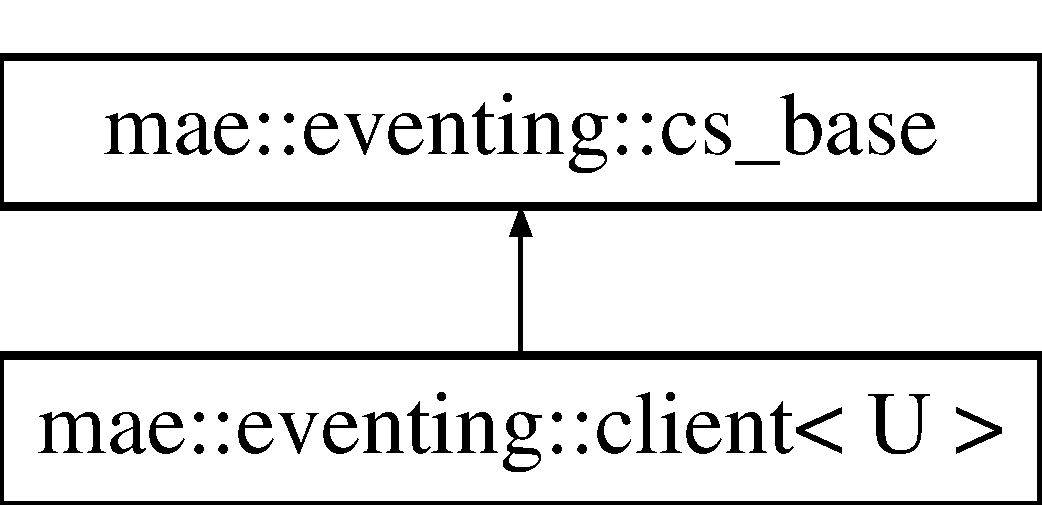
\includegraphics[height=2.000000cm]{classmae_1_1eventing_1_1client}
\end{center}
\end{figure}
\subsection*{Public Member Functions}
\begin{DoxyCompactItemize}
\item 
\hyperlink{classmae_1_1eventing_1_1client_a373432ccb417f31d7e9d63bd7f85c315}{client} (std\-::shared\-\_\-ptr$<$ \hyperlink{classmae_1_1eventing_1_1i__sequence__serializer}{i\-\_\-sequence\-\_\-serializer}$<$ U $>$ $>$ serializer, std\-::string uri, uint16\-\_\-t port=\hyperlink{classmae_1_1eventing_1_1cs__base_a5c068f50b548ec7299133976c00fa5a4}{cs\-\_\-base\-::get\-\_\-default\-\_\-port}(), std\-::string password=\char`\"{}\char`\"{}, bool short\-\_\-sequences=false)
\item 
virtual void \hyperlink{classmae_1_1eventing_1_1client_a8d6b202397c1f209a7eb06f0270e26e7}{register\-\_\-sequence} (std\-::shared\-\_\-ptr$<$ U $>$ sequence)
\item 
virtual void \hyperlink{classmae_1_1eventing_1_1client_a386bcfe7d090b991ed4949856b092a67}{add\-\_\-listener} (std\-::shared\-\_\-ptr$<$ i\-\_\-recognition\-\_\-listener$<$ U $>$ $>$ recognition\-\_\-listener)
\item 
virtual bool \hyperlink{classmae_1_1eventing_1_1client_a929df1715e36580d2233413c2ea3224a}{remove\-\_\-listener} (std\-::shared\-\_\-ptr$<$ i\-\_\-recognition\-\_\-listener$<$ U $>$ $>$ recognition\-\_\-listener)
\item 
virtual std\-::list\\*
$<$ std\-::shared\-\_\-ptr\\*
$<$ i\-\_\-recognition\-\_\-listener$<$ U $>$ $>$ $>$ \hyperlink{classmae_1_1eventing_1_1client_a89ba2ddd24cda5f89efdea85ce01c82d}{get\-\_\-listeners} ()
\item 
virtual void \hyperlink{classmae_1_1eventing_1_1client_a787a1fb0b964d99676ce2a1da0a0c4fe}{notify\-\_\-listeners} (long timestamp, std\-::vector$<$ std\-::shared\-\_\-ptr$<$ U $>$ $>$ sequences)
\item 
virtual void \hyperlink{classmae_1_1eventing_1_1client_a46e28e540f0d823059268e1a275afe0e}{notify\-\_\-listeners} (long timestamp, std\-::vector$<$ std\-::string $>$ sequences\-\_\-titles)
\end{DoxyCompactItemize}
\subsection*{Protected Member Functions}
\begin{DoxyCompactItemize}
\item 
virtual void \hyperlink{classmae_1_1eventing_1_1client_af59c56506b948ba536c3a2fed52daa43}{handle\-\_\-recognition\-\_\-message} (std\-::string message, bool short\-\_\-type)
\item 
virtual std\-::string \hyperlink{classmae_1_1eventing_1_1client_ad205daba9f3fe6834a229e232b0764bc}{create\-\_\-initial\-\_\-message} (bool short\-\_\-type, std\-::string client\-\_\-password)
\item 
virtual std\-::string \hyperlink{classmae_1_1eventing_1_1client_a5f450631a5f2df1e7d990cd7db946a7f}{create\-\_\-registration\-\_\-message} (std\-::shared\-\_\-ptr$<$ U $>$ sequence)
\item 
virtual void \hyperlink{classmae_1_1eventing_1_1client_a9b4b9b0cc974811fd4f2386c35aa13ab}{remove\-\_\-connection} (std\-::shared\-\_\-ptr$<$ boost\-::asio\-::ip\-::tcp\-::socket $>$ connection)
\end{DoxyCompactItemize}
\subsection*{Additional Inherited Members}


\subsection{Constructor \& Destructor Documentation}
\hypertarget{classmae_1_1eventing_1_1client_a373432ccb417f31d7e9d63bd7f85c315}{\index{mae\-::eventing\-::client@{mae\-::eventing\-::client}!client@{client}}
\index{client@{client}!mae::eventing::client@{mae\-::eventing\-::client}}
\subsubsection[{client}]{\setlength{\rightskip}{0pt plus 5cm}template$<$typename U$>$ {\bf mae\-::eventing\-::client}$<$ U $>$\-::{\bf client} (
\begin{DoxyParamCaption}
\item[{std\-::shared\-\_\-ptr$<$ {\bf i\-\_\-sequence\-\_\-serializer}$<$ U $>$ $>$}]{serializer, }
\item[{std\-::string}]{uri, }
\item[{uint16\-\_\-t}]{port = {\ttfamily {\bf cs\-\_\-base\-::get\-\_\-default\-\_\-port}()}, }
\item[{std\-::string}]{password = {\ttfamily \char`\"{}\char`\"{}}, }
\item[{bool}]{short\-\_\-sequences = {\ttfamily false}}
\end{DoxyParamCaption}
)}}\label{classmae_1_1eventing_1_1client_a373432ccb417f31d7e9d63bd7f85c315}
Creates a new client that connects to the server.


\begin{DoxyParams}{Parameters}
{\em serializer} & The serializer used to parse and serialze sequences. \\
\hline
{\em uri} & The server's address (I\-P). \\
\hline
{\em port} & The port on which the server operates. \\
\hline
{\em password} & The password for the server. \\
\hline
{\em short\-\_\-sequences} & True for short sequences (e.\-g. only titles). \\
\hline
\end{DoxyParams}


\subsection{Member Function Documentation}
\hypertarget{classmae_1_1eventing_1_1client_a386bcfe7d090b991ed4949856b092a67}{\index{mae\-::eventing\-::client@{mae\-::eventing\-::client}!add\-\_\-listener@{add\-\_\-listener}}
\index{add\-\_\-listener@{add\-\_\-listener}!mae::eventing::client@{mae\-::eventing\-::client}}
\subsubsection[{add\-\_\-listener}]{\setlength{\rightskip}{0pt plus 5cm}template$<$typename U$>$ void {\bf mae\-::eventing\-::client}$<$ U $>$\-::add\-\_\-listener (
\begin{DoxyParamCaption}
\item[{std\-::shared\-\_\-ptr$<$ i\-\_\-recognition\-\_\-listener$<$ U $>$ $>$}]{recognition\-\_\-listener}
\end{DoxyParamCaption}
)\hspace{0.3cm}{\ttfamily [virtual]}}}\label{classmae_1_1eventing_1_1client_a386bcfe7d090b991ed4949856b092a67}
Adds a listener to the client which is invoked whenever a recognition event is distributed.


\begin{DoxyParams}{Parameters}
{\em recognition\-\_\-listener} & The listener. \\
\hline
\end{DoxyParams}
\hypertarget{classmae_1_1eventing_1_1client_ad205daba9f3fe6834a229e232b0764bc}{\index{mae\-::eventing\-::client@{mae\-::eventing\-::client}!create\-\_\-initial\-\_\-message@{create\-\_\-initial\-\_\-message}}
\index{create\-\_\-initial\-\_\-message@{create\-\_\-initial\-\_\-message}!mae::eventing::client@{mae\-::eventing\-::client}}
\subsubsection[{create\-\_\-initial\-\_\-message}]{\setlength{\rightskip}{0pt plus 5cm}template$<$typename U $>$ std\-::string {\bf mae\-::eventing\-::client}$<$ U $>$\-::create\-\_\-initial\-\_\-message (
\begin{DoxyParamCaption}
\item[{bool}]{short\-\_\-type, }
\item[{std\-::string}]{client\-\_\-password}
\end{DoxyParamCaption}
)\hspace{0.3cm}{\ttfamily [protected]}, {\ttfamily [virtual]}}}\label{classmae_1_1eventing_1_1client_ad205daba9f3fe6834a229e232b0764bc}
Generates the initial message which is sent to the server in order to establish a connection.


\begin{DoxyParams}{Parameters}
{\em short\-\_\-type} & The message type to be received. True for short. \\
\hline
\end{DoxyParams}
\begin{DoxyReturn}{Returns}
The message string. 
\end{DoxyReturn}
\hypertarget{classmae_1_1eventing_1_1client_a5f450631a5f2df1e7d990cd7db946a7f}{\index{mae\-::eventing\-::client@{mae\-::eventing\-::client}!create\-\_\-registration\-\_\-message@{create\-\_\-registration\-\_\-message}}
\index{create\-\_\-registration\-\_\-message@{create\-\_\-registration\-\_\-message}!mae::eventing::client@{mae\-::eventing\-::client}}
\subsubsection[{create\-\_\-registration\-\_\-message}]{\setlength{\rightskip}{0pt plus 5cm}template$<$typename U$>$ std\-::string {\bf mae\-::eventing\-::client}$<$ U $>$\-::create\-\_\-registration\-\_\-message (
\begin{DoxyParamCaption}
\item[{std\-::shared\-\_\-ptr$<$ U $>$}]{sequence}
\end{DoxyParamCaption}
)\hspace{0.3cm}{\ttfamily [protected]}, {\ttfamily [virtual]}}}\label{classmae_1_1eventing_1_1client_a5f450631a5f2df1e7d990cd7db946a7f}
Generates the registration message which is sent to the server in order to register another sequence to the movement controller. This message contains always the whole sequence representation in order to be constructed at the server.


\begin{DoxyParams}{Parameters}
{\em sequence} & The sequence. \\
\hline
\end{DoxyParams}
\begin{DoxyReturn}{Returns}
The message string. 
\end{DoxyReturn}
\hypertarget{classmae_1_1eventing_1_1client_a89ba2ddd24cda5f89efdea85ce01c82d}{\index{mae\-::eventing\-::client@{mae\-::eventing\-::client}!get\-\_\-listeners@{get\-\_\-listeners}}
\index{get\-\_\-listeners@{get\-\_\-listeners}!mae::eventing::client@{mae\-::eventing\-::client}}
\subsubsection[{get\-\_\-listeners}]{\setlength{\rightskip}{0pt plus 5cm}template$<$typename U $>$ std\-::list$<$ std\-::shared\-\_\-ptr$<$ i\-\_\-recognition\-\_\-listener$<$ U $>$ $>$ $>$ {\bf mae\-::eventing\-::client}$<$ U $>$\-::get\-\_\-listeners (
\begin{DoxyParamCaption}
{}
\end{DoxyParamCaption}
)\hspace{0.3cm}{\ttfamily [virtual]}}}\label{classmae_1_1eventing_1_1client_a89ba2ddd24cda5f89efdea85ce01c82d}
Returns all registered listeners.

\begin{DoxyReturn}{Returns}
The listeners. 
\end{DoxyReturn}
\hypertarget{classmae_1_1eventing_1_1client_af59c56506b948ba536c3a2fed52daa43}{\index{mae\-::eventing\-::client@{mae\-::eventing\-::client}!handle\-\_\-recognition\-\_\-message@{handle\-\_\-recognition\-\_\-message}}
\index{handle\-\_\-recognition\-\_\-message@{handle\-\_\-recognition\-\_\-message}!mae::eventing::client@{mae\-::eventing\-::client}}
\subsubsection[{handle\-\_\-recognition\-\_\-message}]{\setlength{\rightskip}{0pt plus 5cm}template$<$typename U $>$ void {\bf mae\-::eventing\-::client}$<$ U $>$\-::handle\-\_\-recognition\-\_\-message (
\begin{DoxyParamCaption}
\item[{std\-::string}]{message, }
\item[{bool}]{short\-\_\-type}
\end{DoxyParamCaption}
)\hspace{0.3cm}{\ttfamily [protected]}, {\ttfamily [virtual]}}}\label{classmae_1_1eventing_1_1client_af59c56506b948ba536c3a2fed52daa43}
Handles the message which contains information on recognized sequences. Is invoked whenever a message was completely read from the stream. From this method the specific notify\-\_\-listeners-\/method is invoked.


\begin{DoxyParams}{Parameters}
{\em message} & The message to be parsed \\
\hline
\end{DoxyParams}
\hypertarget{classmae_1_1eventing_1_1client_a787a1fb0b964d99676ce2a1da0a0c4fe}{\index{mae\-::eventing\-::client@{mae\-::eventing\-::client}!notify\-\_\-listeners@{notify\-\_\-listeners}}
\index{notify\-\_\-listeners@{notify\-\_\-listeners}!mae::eventing::client@{mae\-::eventing\-::client}}
\subsubsection[{notify\-\_\-listeners}]{\setlength{\rightskip}{0pt plus 5cm}template$<$typename U$>$ void {\bf mae\-::eventing\-::client}$<$ U $>$\-::notify\-\_\-listeners (
\begin{DoxyParamCaption}
\item[{long}]{timestamp, }
\item[{std\-::vector$<$ std\-::shared\-\_\-ptr$<$ U $>$ $>$}]{sequences}
\end{DoxyParamCaption}
)\hspace{0.3cm}{\ttfamily [virtual]}}}\label{classmae_1_1eventing_1_1client_a787a1fb0b964d99676ce2a1da0a0c4fe}
Notifies the listeners on a recognized sequence.


\begin{DoxyParams}{Parameters}
{\em timestamp} & The timestamp. \\
\hline
{\em sequences} & The sequences. \\
\hline
\end{DoxyParams}
\hypertarget{classmae_1_1eventing_1_1client_a46e28e540f0d823059268e1a275afe0e}{\index{mae\-::eventing\-::client@{mae\-::eventing\-::client}!notify\-\_\-listeners@{notify\-\_\-listeners}}
\index{notify\-\_\-listeners@{notify\-\_\-listeners}!mae::eventing::client@{mae\-::eventing\-::client}}
\subsubsection[{notify\-\_\-listeners}]{\setlength{\rightskip}{0pt plus 5cm}template$<$typename U$>$ void {\bf mae\-::eventing\-::client}$<$ U $>$\-::notify\-\_\-listeners (
\begin{DoxyParamCaption}
\item[{long}]{timestamp, }
\item[{std\-::vector$<$ std\-::string $>$}]{sequences\-\_\-titles}
\end{DoxyParamCaption}
)\hspace{0.3cm}{\ttfamily [virtual]}}}\label{classmae_1_1eventing_1_1client_a46e28e540f0d823059268e1a275afe0e}
Notifies the listeners on a recognized sequence. Only the sequence titles are provided.


\begin{DoxyParams}{Parameters}
{\em timestamp} & The timestamp. \\
\hline
{\em sequences\-\_\-titles} & The sequence titles. \\
\hline
\end{DoxyParams}
\hypertarget{classmae_1_1eventing_1_1client_a8d6b202397c1f209a7eb06f0270e26e7}{\index{mae\-::eventing\-::client@{mae\-::eventing\-::client}!register\-\_\-sequence@{register\-\_\-sequence}}
\index{register\-\_\-sequence@{register\-\_\-sequence}!mae::eventing::client@{mae\-::eventing\-::client}}
\subsubsection[{register\-\_\-sequence}]{\setlength{\rightskip}{0pt plus 5cm}template$<$typename U$>$ void {\bf mae\-::eventing\-::client}$<$ U $>$\-::register\-\_\-sequence (
\begin{DoxyParamCaption}
\item[{std\-::shared\-\_\-ptr$<$ U $>$}]{sequence}
\end{DoxyParamCaption}
)\hspace{0.3cm}{\ttfamily [virtual]}}}\label{classmae_1_1eventing_1_1client_a8d6b202397c1f209a7eb06f0270e26e7}
Registers another sequence to the server side.


\begin{DoxyParams}{Parameters}
{\em sequence} & The sequence to be registered. \\
\hline
\end{DoxyParams}
\hypertarget{classmae_1_1eventing_1_1client_a9b4b9b0cc974811fd4f2386c35aa13ab}{\index{mae\-::eventing\-::client@{mae\-::eventing\-::client}!remove\-\_\-connection@{remove\-\_\-connection}}
\index{remove\-\_\-connection@{remove\-\_\-connection}!mae::eventing::client@{mae\-::eventing\-::client}}
\subsubsection[{remove\-\_\-connection}]{\setlength{\rightskip}{0pt plus 5cm}template$<$typename U $>$ void {\bf mae\-::eventing\-::client}$<$ U $>$\-::remove\-\_\-connection (
\begin{DoxyParamCaption}
\item[{std\-::shared\-\_\-ptr$<$ boost\-::asio\-::ip\-::tcp\-::socket $>$}]{connection}
\end{DoxyParamCaption}
)\hspace{0.3cm}{\ttfamily [protected]}, {\ttfamily [virtual]}}}\label{classmae_1_1eventing_1_1client_a9b4b9b0cc974811fd4f2386c35aa13ab}
Closes the connection to the server.


\begin{DoxyParams}{Parameters}
{\em connection} & The connection. \\
\hline
\end{DoxyParams}
\hypertarget{classmae_1_1eventing_1_1client_a929df1715e36580d2233413c2ea3224a}{\index{mae\-::eventing\-::client@{mae\-::eventing\-::client}!remove\-\_\-listener@{remove\-\_\-listener}}
\index{remove\-\_\-listener@{remove\-\_\-listener}!mae::eventing::client@{mae\-::eventing\-::client}}
\subsubsection[{remove\-\_\-listener}]{\setlength{\rightskip}{0pt plus 5cm}template$<$typename U$>$ bool {\bf mae\-::eventing\-::client}$<$ U $>$\-::remove\-\_\-listener (
\begin{DoxyParamCaption}
\item[{std\-::shared\-\_\-ptr$<$ i\-\_\-recognition\-\_\-listener$<$ U $>$ $>$}]{recognition\-\_\-listener}
\end{DoxyParamCaption}
)\hspace{0.3cm}{\ttfamily [virtual]}}}\label{classmae_1_1eventing_1_1client_a929df1715e36580d2233413c2ea3224a}
Removes the listener from the client.


\begin{DoxyParams}{Parameters}
{\em recognition\-\_\-listener} & The listener. \\
\hline
\end{DoxyParams}
\begin{DoxyReturn}{Returns}
True on success. 
\end{DoxyReturn}


The documentation for this class was generated from the following file\-:\begin{DoxyCompactItemize}
\item 
src/mae/eventing/client.\-hpp\end{DoxyCompactItemize}

\hypertarget{classmae_1_1eventing_1_1cs__base}{\section{mae\-:\-:eventing\-:\-:cs\-\_\-base Class Reference}
\label{classmae_1_1eventing_1_1cs__base}\index{mae\-::eventing\-::cs\-\_\-base@{mae\-::eventing\-::cs\-\_\-base}}
}
Inheritance diagram for mae\-:\-:eventing\-:\-:cs\-\_\-base\-:\begin{figure}[H]
\begin{center}
\leavevmode
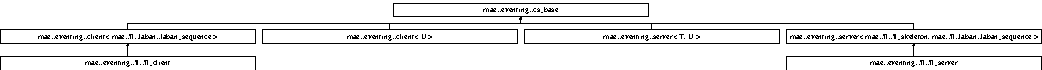
\includegraphics[height=0.941704cm]{classmae_1_1eventing_1_1cs__base}
\end{center}
\end{figure}
\subsection*{Public Member Functions}
\begin{DoxyCompactItemize}
\item 
\hyperlink{classmae_1_1eventing_1_1cs__base_ae51b46ccd805bd00ad4dc00fbb9e701b}{cs\-\_\-base} ()
\item 
virtual bool \hyperlink{classmae_1_1eventing_1_1cs__base_a4819997a46dcbf1bba127e02a9cb9c7d}{is\-\_\-message\-\_\-complete} (const std\-::string \&message) const 
\end{DoxyCompactItemize}
\subsection*{Static Public Member Functions}
\begin{DoxyCompactItemize}
\item 
static uint16\-\_\-t \hyperlink{classmae_1_1eventing_1_1cs__base_a5c068f50b548ec7299133976c00fa5a4}{get\-\_\-default\-\_\-port} ()
\end{DoxyCompactItemize}


\subsection{Constructor \& Destructor Documentation}
\hypertarget{classmae_1_1eventing_1_1cs__base_ae51b46ccd805bd00ad4dc00fbb9e701b}{\index{mae\-::eventing\-::cs\-\_\-base@{mae\-::eventing\-::cs\-\_\-base}!cs\-\_\-base@{cs\-\_\-base}}
\index{cs\-\_\-base@{cs\-\_\-base}!mae::eventing::cs_base@{mae\-::eventing\-::cs\-\_\-base}}
\subsubsection[{cs\-\_\-base}]{\setlength{\rightskip}{0pt plus 5cm}mae\-::eventing\-::cs\-\_\-base\-::cs\-\_\-base (
\begin{DoxyParamCaption}
{}
\end{DoxyParamCaption}
)}}\label{classmae_1_1eventing_1_1cs__base_ae51b46ccd805bd00ad4dc00fbb9e701b}
Creates a server base from which the server inherits. 

\subsection{Member Function Documentation}
\hypertarget{classmae_1_1eventing_1_1cs__base_a5c068f50b548ec7299133976c00fa5a4}{\index{mae\-::eventing\-::cs\-\_\-base@{mae\-::eventing\-::cs\-\_\-base}!get\-\_\-default\-\_\-port@{get\-\_\-default\-\_\-port}}
\index{get\-\_\-default\-\_\-port@{get\-\_\-default\-\_\-port}!mae::eventing::cs_base@{mae\-::eventing\-::cs\-\_\-base}}
\subsubsection[{get\-\_\-default\-\_\-port}]{\setlength{\rightskip}{0pt plus 5cm}uint16\-\_\-t mae\-::eventing\-::cs\-\_\-base\-::get\-\_\-default\-\_\-port (
\begin{DoxyParamCaption}
{}
\end{DoxyParamCaption}
)\hspace{0.3cm}{\ttfamily [static]}}}\label{classmae_1_1eventing_1_1cs__base_a5c068f50b548ec7299133976c00fa5a4}
Returns the default port used by the server if no other is specified.

\begin{DoxyReturn}{Returns}
The default port. 
\end{DoxyReturn}
\hypertarget{classmae_1_1eventing_1_1cs__base_a4819997a46dcbf1bba127e02a9cb9c7d}{\index{mae\-::eventing\-::cs\-\_\-base@{mae\-::eventing\-::cs\-\_\-base}!is\-\_\-message\-\_\-complete@{is\-\_\-message\-\_\-complete}}
\index{is\-\_\-message\-\_\-complete@{is\-\_\-message\-\_\-complete}!mae::eventing::cs_base@{mae\-::eventing\-::cs\-\_\-base}}
\subsubsection[{is\-\_\-message\-\_\-complete}]{\setlength{\rightskip}{0pt plus 5cm}bool mae\-::eventing\-::cs\-\_\-base\-::is\-\_\-message\-\_\-complete (
\begin{DoxyParamCaption}
\item[{const std\-::string \&}]{message}
\end{DoxyParamCaption}
) const\hspace{0.3cm}{\ttfamily [virtual]}}}\label{classmae_1_1eventing_1_1cs__base_a4819997a46dcbf1bba127e02a9cb9c7d}
Checks whether the sent message is complete. Returns true if that is the case. Returns false otherwise.


\begin{DoxyParams}{Parameters}
{\em message} & The message to be checked for completeness. \\
\hline
\end{DoxyParams}
\begin{DoxyReturn}{Returns}
True if complete. 
\end{DoxyReturn}


The documentation for this class was generated from the following files\-:\begin{DoxyCompactItemize}
\item 
src/mae/eventing/cs\-\_\-base.\-hpp\item 
src/mae/eventing/cs\-\_\-base.\-cpp\end{DoxyCompactItemize}

\hypertarget{classmae_1_1eventing_1_1fl_1_1fl__client}{\section{mae\-:\-:eventing\-:\-:fl\-:\-:fl\-\_\-client Class Reference}
\label{classmae_1_1eventing_1_1fl_1_1fl__client}\index{mae\-::eventing\-::fl\-::fl\-\_\-client@{mae\-::eventing\-::fl\-::fl\-\_\-client}}
}
Inheritance diagram for mae\-:\-:eventing\-:\-:fl\-:\-:fl\-\_\-client\-:\begin{figure}[H]
\begin{center}
\leavevmode
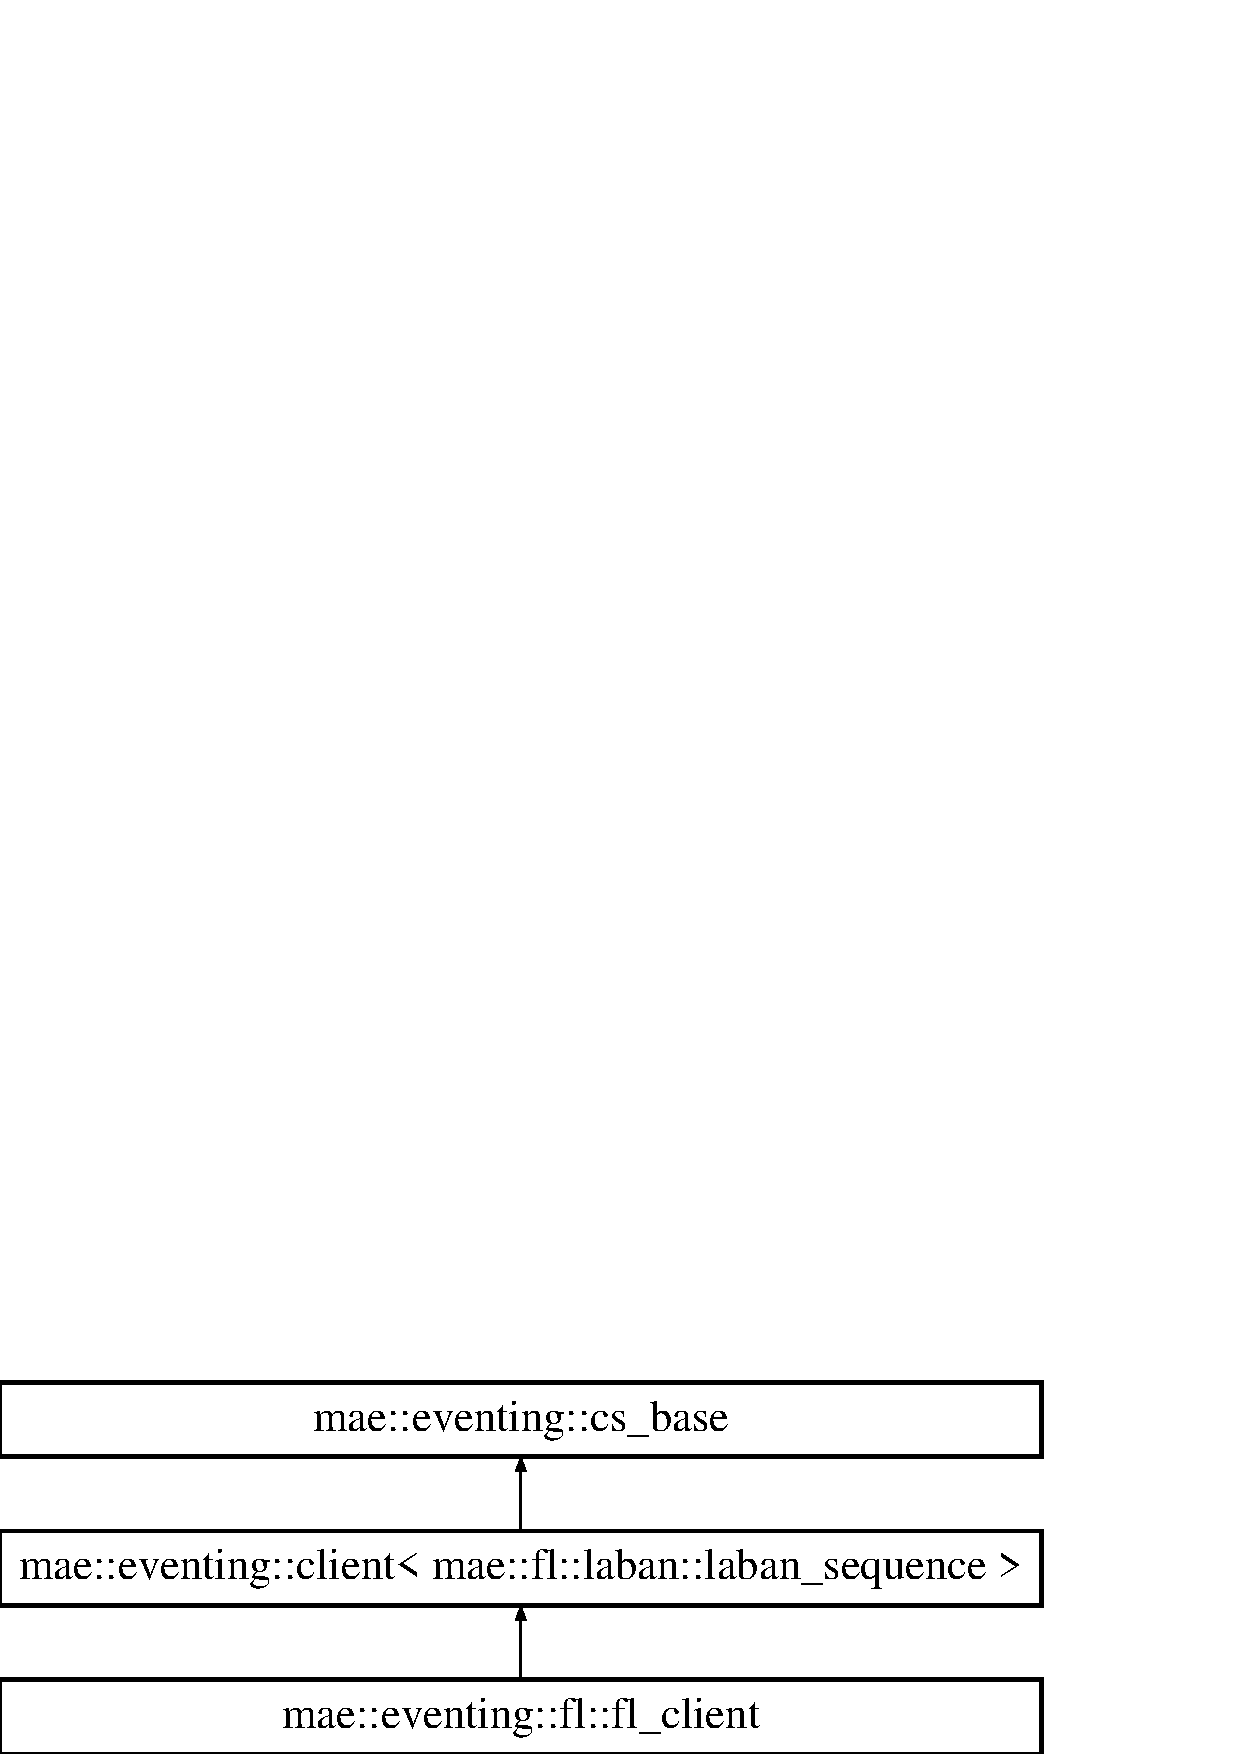
\includegraphics[height=3.000000cm]{classmae_1_1eventing_1_1fl_1_1fl__client}
\end{center}
\end{figure}
\subsection*{Public Member Functions}
\begin{DoxyCompactItemize}
\item 
\hyperlink{classmae_1_1eventing_1_1fl_1_1fl__client_a76156e6e8b7a6703115d7f2d6aa76e78}{fl\-\_\-client} (std\-::string uri, uint16\-\_\-t port=\hyperlink{classmae_1_1eventing_1_1cs__base_a5c068f50b548ec7299133976c00fa5a4}{cs\-\_\-base\-::get\-\_\-default\-\_\-port}(), std\-::string password=\char`\"{}\char`\"{}, bool short\-\_\-sequences=false, bool debug=false)
\end{DoxyCompactItemize}
\subsection*{Additional Inherited Members}


\subsection{Constructor \& Destructor Documentation}
\hypertarget{classmae_1_1eventing_1_1fl_1_1fl__client_a76156e6e8b7a6703115d7f2d6aa76e78}{\index{mae\-::eventing\-::fl\-::fl\-\_\-client@{mae\-::eventing\-::fl\-::fl\-\_\-client}!fl\-\_\-client@{fl\-\_\-client}}
\index{fl\-\_\-client@{fl\-\_\-client}!mae::eventing::fl::fl_client@{mae\-::eventing\-::fl\-::fl\-\_\-client}}
\subsubsection[{fl\-\_\-client}]{\setlength{\rightskip}{0pt plus 5cm}mae\-::eventing\-::fl\-::fl\-\_\-client\-::fl\-\_\-client (
\begin{DoxyParamCaption}
\item[{std\-::string}]{uri, }
\item[{uint16\-\_\-t}]{port = {\ttfamily {\bf cs\-\_\-base\-::get\-\_\-default\-\_\-port}()}, }
\item[{std\-::string}]{password = {\ttfamily \char`\"{}\char`\"{}}, }
\item[{bool}]{short\-\_\-sequences = {\ttfamily false}, }
\item[{bool}]{debug = {\ttfamily false}}
\end{DoxyParamCaption}
)}}\label{classmae_1_1eventing_1_1fl_1_1fl__client_a76156e6e8b7a6703115d7f2d6aa76e78}
Creates a new client which works with laban sequences.


\begin{DoxyParams}{Parameters}
{\em uri} & The uri of the server to connect to (I\-P address) \\
\hline
{\em port} & The port to be connected to. \\
\hline
{\em password} & The server password. \\
\hline
{\em short\-\_\-sequences} & True if sequences shall be of short format (only sequence titles). \\
\hline
{\em debug} & True for debug output. \\
\hline
\end{DoxyParams}


The documentation for this class was generated from the following files\-:\begin{DoxyCompactItemize}
\item 
src/mae/eventing/fl/fl\-\_\-client.\-hpp\item 
src/mae/eventing/fl/fl\-\_\-client.\-cpp\end{DoxyCompactItemize}

\hypertarget{classmae_1_1eventing_1_1fl_1_1fl__server}{\section{mae\-:\-:eventing\-:\-:fl\-:\-:fl\-\_\-server Class Reference}
\label{classmae_1_1eventing_1_1fl_1_1fl__server}\index{mae\-::eventing\-::fl\-::fl\-\_\-server@{mae\-::eventing\-::fl\-::fl\-\_\-server}}
}
Inheritance diagram for mae\-:\-:eventing\-:\-:fl\-:\-:fl\-\_\-server\-:\begin{figure}[H]
\begin{center}
\leavevmode
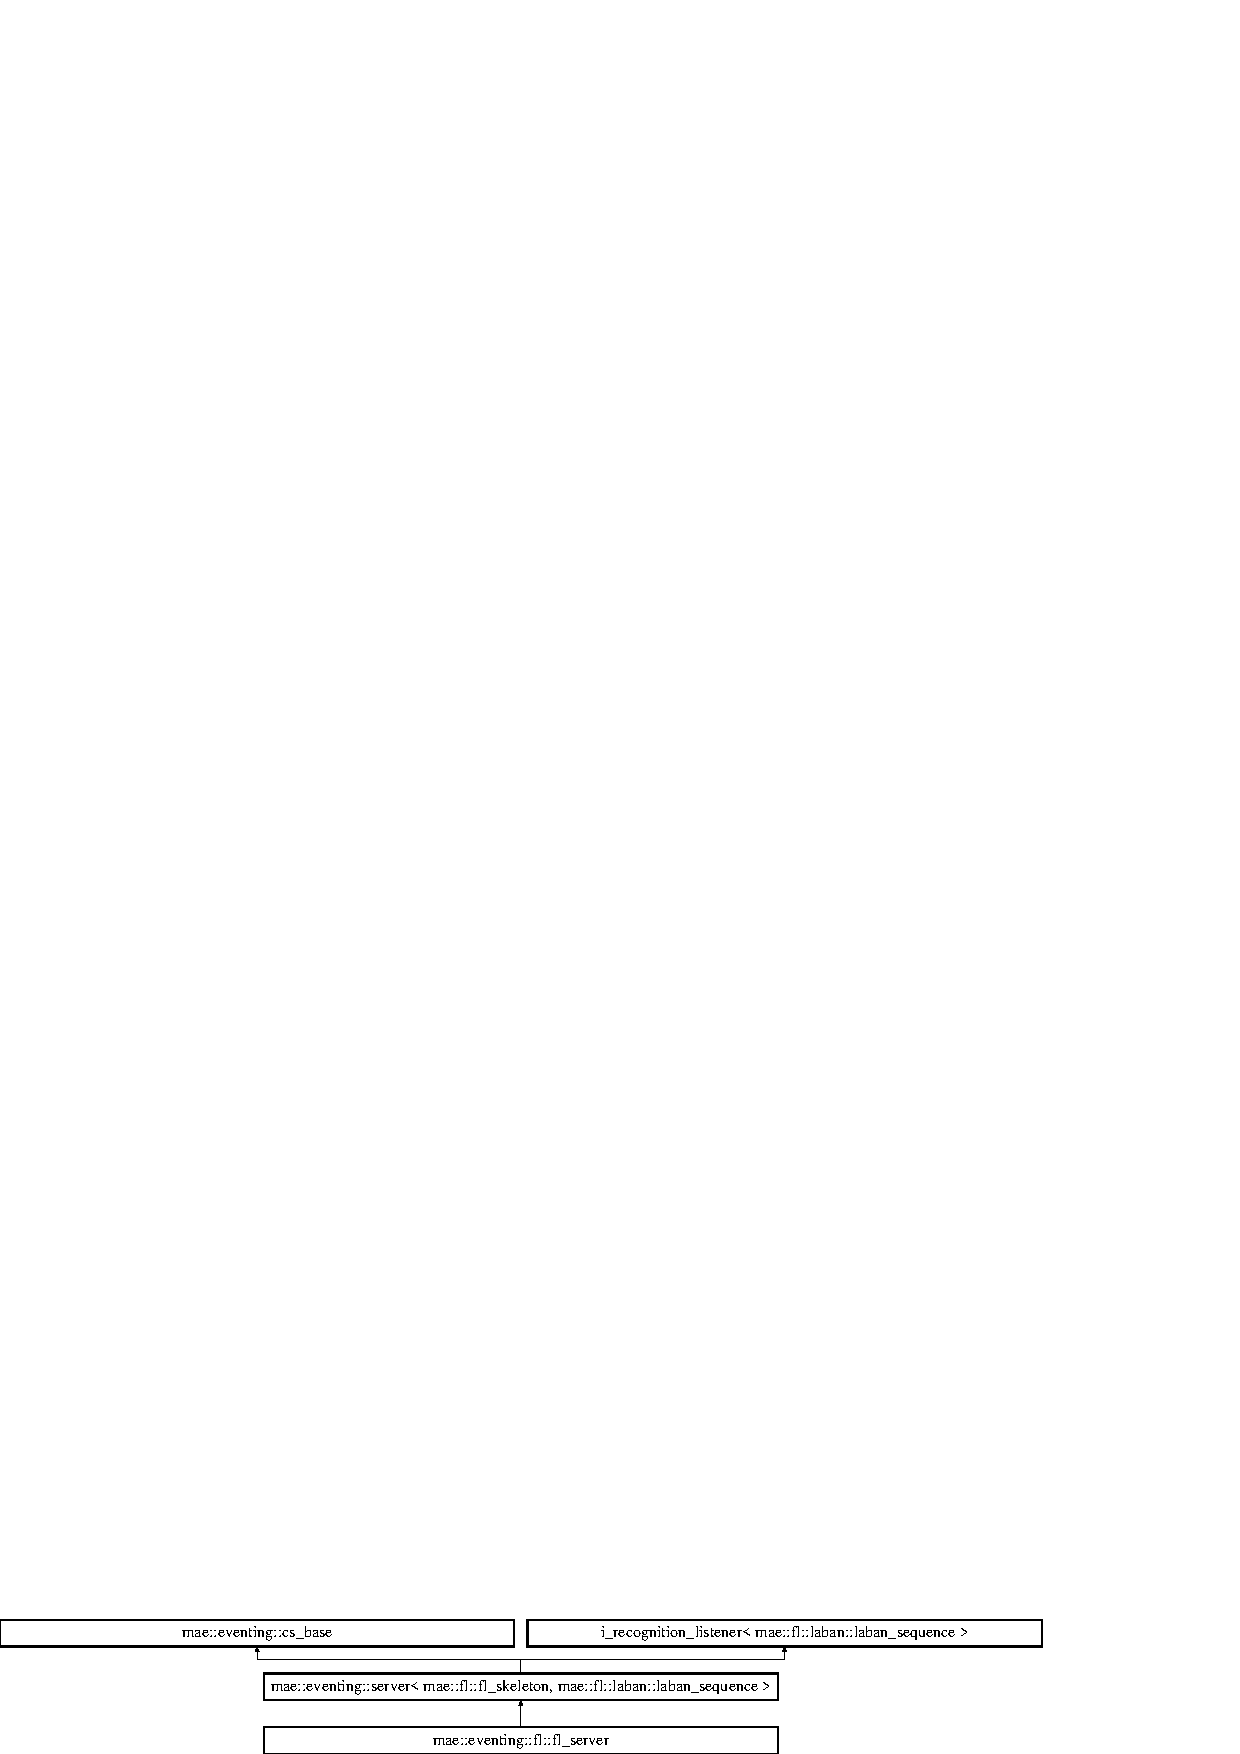
\includegraphics[height=1.883408cm]{classmae_1_1eventing_1_1fl_1_1fl__server}
\end{center}
\end{figure}
\subsection*{Public Member Functions}
\begin{DoxyCompactItemize}
\item 
\hyperlink{classmae_1_1eventing_1_1fl_1_1fl__server_a6358c3106e583a068508b97146aa3408}{fl\-\_\-server} (mae\-::fl\-::fl\-\_\-movement\-\_\-controller $\ast$mov\-\_\-controller=nullptr, uint16\-\_\-t port=\hyperlink{classmae_1_1eventing_1_1cs__base_a5c068f50b548ec7299133976c00fa5a4}{cs\-\_\-base\-::get\-\_\-default\-\_\-port}(), std\-::string password=\char`\"{}\char`\"{})
\end{DoxyCompactItemize}
\subsection*{Additional Inherited Members}


\subsection{Constructor \& Destructor Documentation}
\hypertarget{classmae_1_1eventing_1_1fl_1_1fl__server_a6358c3106e583a068508b97146aa3408}{\index{mae\-::eventing\-::fl\-::fl\-\_\-server@{mae\-::eventing\-::fl\-::fl\-\_\-server}!fl\-\_\-server@{fl\-\_\-server}}
\index{fl\-\_\-server@{fl\-\_\-server}!mae::eventing::fl::fl_server@{mae\-::eventing\-::fl\-::fl\-\_\-server}}
\subsubsection[{fl\-\_\-server}]{\setlength{\rightskip}{0pt plus 5cm}mae\-::eventing\-::fl\-::fl\-\_\-server\-::fl\-\_\-server (
\begin{DoxyParamCaption}
\item[{mae\-::fl\-::fl\-\_\-movement\-\_\-controller $\ast$}]{mov\-\_\-controller = {\ttfamily nullptr}, }
\item[{uint16\-\_\-t}]{port = {\ttfamily {\bf cs\-\_\-base\-::get\-\_\-default\-\_\-port}()}, }
\item[{std\-::string}]{password = {\ttfamily \char`\"{}\char`\"{}}}
\end{DoxyParamCaption}
)}}\label{classmae_1_1eventing_1_1fl_1_1fl__server_a6358c3106e583a068508b97146aa3408}
Creates a new server which works with laban sequences and fl skeletons.


\begin{DoxyParams}{Parameters}
{\em mov\-\_\-controller} & The movement controller to which sequences are registered if any received from a client. \\
\hline
{\em port} & The port to be worked on. \\
\hline
{\em password} & The server password. \\
\hline
\end{DoxyParams}


The documentation for this class was generated from the following files\-:\begin{DoxyCompactItemize}
\item 
src/mae/eventing/fl/fl\-\_\-server.\-hpp\item 
src/mae/eventing/fl/fl\-\_\-server.\-cpp\end{DoxyCompactItemize}

\hypertarget{classmae_1_1eventing_1_1i__registration__manager}{\section{mae\-:\-:eventing\-:\-:i\-\_\-registration\-\_\-manager$<$ U $>$ Class Template Reference}
\label{classmae_1_1eventing_1_1i__registration__manager}\index{mae\-::eventing\-::i\-\_\-registration\-\_\-manager$<$ U $>$@{mae\-::eventing\-::i\-\_\-registration\-\_\-manager$<$ U $>$}}
}
\subsection*{Public Member Functions}
\begin{DoxyCompactItemize}
\item 
virtual bool \hyperlink{classmae_1_1eventing_1_1i__registration__manager_ac0490911c233d6ad7f65652b35c57cb1}{on\-\_\-sequence\-\_\-registered} (std\-::shared\-\_\-ptr$<$ U $>$ sequence)=0
\end{DoxyCompactItemize}


\subsection{Member Function Documentation}
\hypertarget{classmae_1_1eventing_1_1i__registration__manager_ac0490911c233d6ad7f65652b35c57cb1}{\index{mae\-::eventing\-::i\-\_\-registration\-\_\-manager@{mae\-::eventing\-::i\-\_\-registration\-\_\-manager}!on\-\_\-sequence\-\_\-registered@{on\-\_\-sequence\-\_\-registered}}
\index{on\-\_\-sequence\-\_\-registered@{on\-\_\-sequence\-\_\-registered}!mae::eventing::i_registration_manager@{mae\-::eventing\-::i\-\_\-registration\-\_\-manager}}
\subsubsection[{on\-\_\-sequence\-\_\-registered}]{\setlength{\rightskip}{0pt plus 5cm}template$<$typename U $>$ virtual bool {\bf mae\-::eventing\-::i\-\_\-registration\-\_\-manager}$<$ U $>$\-::on\-\_\-sequence\-\_\-registered (
\begin{DoxyParamCaption}
\item[{std\-::shared\-\_\-ptr$<$ U $>$}]{sequence}
\end{DoxyParamCaption}
)\hspace{0.3cm}{\ttfamily [pure virtual]}}}\label{classmae_1_1eventing_1_1i__registration__manager_ac0490911c233d6ad7f65652b35c57cb1}
Handles a newly registered sequence which was sent to the server.


\begin{DoxyParams}{Parameters}
{\em sequence} & The received sequence. \\
\hline
\end{DoxyParams}
\begin{DoxyReturn}{Returns}
True if the sequence is intended to be added to the movement controller. False otherwise. 
\end{DoxyReturn}


The documentation for this class was generated from the following file\-:\begin{DoxyCompactItemize}
\item 
src/mae/eventing/i\-\_\-registration\-\_\-manager.\-hpp\end{DoxyCompactItemize}

\hypertarget{classmae_1_1eventing_1_1i__sequence__serializer}{\section{mae\-:\-:eventing\-:\-:i\-\_\-sequence\-\_\-serializer$<$ U $>$ Class Template Reference}
\label{classmae_1_1eventing_1_1i__sequence__serializer}\index{mae\-::eventing\-::i\-\_\-sequence\-\_\-serializer$<$ U $>$@{mae\-::eventing\-::i\-\_\-sequence\-\_\-serializer$<$ U $>$}}
}
\subsection*{Public Member Functions}
\begin{DoxyCompactItemize}
\item 
virtual std\-::string \hyperlink{classmae_1_1eventing_1_1i__sequence__serializer_a82204865ed1a9372dc67a3e67a8681e6}{serialize} (std\-::shared\-\_\-ptr$<$ U $>$ sequence, bool short\-\_\-type, bool no\-\_\-header=false, unsigned int indent=0, std\-::string namesp=\char`\"{}laban\char`\"{})=0
\item 
virtual std\-::shared\-\_\-ptr$<$ U $>$ \hyperlink{classmae_1_1eventing_1_1i__sequence__serializer_ad4b9b90fbaa232a0601956c93a4c407b}{deserialize} (std\-::string sequence)=0
\end{DoxyCompactItemize}


\subsection{Member Function Documentation}
\hypertarget{classmae_1_1eventing_1_1i__sequence__serializer_ad4b9b90fbaa232a0601956c93a4c407b}{\index{mae\-::eventing\-::i\-\_\-sequence\-\_\-serializer@{mae\-::eventing\-::i\-\_\-sequence\-\_\-serializer}!deserialize@{deserialize}}
\index{deserialize@{deserialize}!mae::eventing::i_sequence_serializer@{mae\-::eventing\-::i\-\_\-sequence\-\_\-serializer}}
\subsubsection[{deserialize}]{\setlength{\rightskip}{0pt plus 5cm}template$<$typename U$>$ virtual std\-::shared\-\_\-ptr$<$U$>$ {\bf mae\-::eventing\-::i\-\_\-sequence\-\_\-serializer}$<$ U $>$\-::deserialize (
\begin{DoxyParamCaption}
\item[{std\-::string}]{sequence}
\end{DoxyParamCaption}
)\hspace{0.3cm}{\ttfamily [pure virtual]}}}\label{classmae_1_1eventing_1_1i__sequence__serializer_ad4b9b90fbaa232a0601956c93a4c407b}
Deserializes the sequence so that it can be registered to the engine.


\begin{DoxyParams}{Parameters}
{\em sequence} & The serialized sequence string. \\
\hline
\end{DoxyParams}
\begin{DoxyReturn}{Returns}
The sequence object. 
\end{DoxyReturn}


Implemented in \hyperlink{classmae_1_1eventing_1_1fl_1_1laban__serializer_a67d675cf407100bfdb05375b27716674}{mae\-::eventing\-::fl\-::laban\-\_\-serializer}.

\hypertarget{classmae_1_1eventing_1_1i__sequence__serializer_a82204865ed1a9372dc67a3e67a8681e6}{\index{mae\-::eventing\-::i\-\_\-sequence\-\_\-serializer@{mae\-::eventing\-::i\-\_\-sequence\-\_\-serializer}!serialize@{serialize}}
\index{serialize@{serialize}!mae::eventing::i_sequence_serializer@{mae\-::eventing\-::i\-\_\-sequence\-\_\-serializer}}
\subsubsection[{serialize}]{\setlength{\rightskip}{0pt plus 5cm}template$<$typename U$>$ virtual std\-::string {\bf mae\-::eventing\-::i\-\_\-sequence\-\_\-serializer}$<$ U $>$\-::serialize (
\begin{DoxyParamCaption}
\item[{std\-::shared\-\_\-ptr$<$ U $>$}]{sequence, }
\item[{bool}]{short\-\_\-type, }
\item[{bool}]{no\-\_\-header = {\ttfamily false}, }
\item[{unsigned int}]{indent = {\ttfamily 0}, }
\item[{std\-::string}]{namesp = {\ttfamily \char`\"{}laban\char`\"{}}}
\end{DoxyParamCaption}
)\hspace{0.3cm}{\ttfamily [pure virtual]}}}\label{classmae_1_1eventing_1_1i__sequence__serializer_a82204865ed1a9372dc67a3e67a8681e6}
Serializes the sequence so that it can be printed to a string.


\begin{DoxyParams}{Parameters}
{\em sequence} & The sequence. \\
\hline
\end{DoxyParams}
\begin{DoxyReturn}{Returns}
The string containing the serialized sequence. 
\end{DoxyReturn}


Implemented in \hyperlink{classmae_1_1eventing_1_1fl_1_1laban__serializer_a8b3e378b2289428fb8511df06b81a18a}{mae\-::eventing\-::fl\-::laban\-\_\-serializer}.



The documentation for this class was generated from the following file\-:\begin{DoxyCompactItemize}
\item 
src/mae/eventing/i\-\_\-sequence\-\_\-serializer.\-hpp\end{DoxyCompactItemize}

\hypertarget{classmae_1_1eventing_1_1fl_1_1laban__serializer}{\section{mae\-:\-:eventing\-:\-:fl\-:\-:laban\-\_\-serializer Class Reference}
\label{classmae_1_1eventing_1_1fl_1_1laban__serializer}\index{mae\-::eventing\-::fl\-::laban\-\_\-serializer@{mae\-::eventing\-::fl\-::laban\-\_\-serializer}}
}
Inheritance diagram for mae\-:\-:eventing\-:\-:fl\-:\-:laban\-\_\-serializer\-:\begin{figure}[H]
\begin{center}
\leavevmode
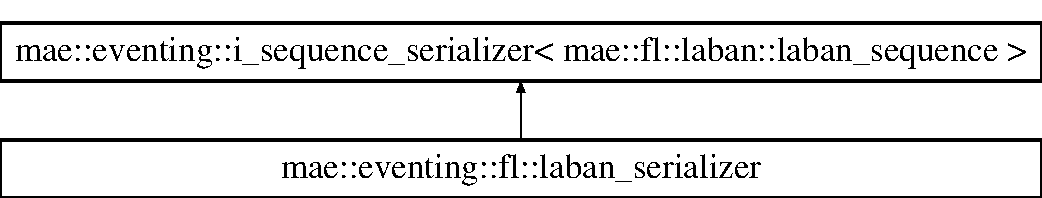
\includegraphics[height=2.000000cm]{classmae_1_1eventing_1_1fl_1_1laban__serializer}
\end{center}
\end{figure}
\subsection*{Public Member Functions}
\begin{DoxyCompactItemize}
\item 
\hyperlink{classmae_1_1eventing_1_1fl_1_1laban__serializer_a03724d2bfeb0bdd28b9ad471d07c1d98}{laban\-\_\-serializer} ()
\item 
virtual std\-::string \hyperlink{classmae_1_1eventing_1_1fl_1_1laban__serializer_a8b3e378b2289428fb8511df06b81a18a}{serialize} (std\-::shared\-\_\-ptr$<$ mae\-::fl\-::laban\-::laban\-\_\-sequence $>$ sequence, bool short\-\_\-type, bool no\-\_\-header=false, unsigned int indent=0, std\-::string namesp=\char`\"{}\char`\"{})
\item 
virtual std\-::shared\-\_\-ptr\\*
$<$ mae\-::fl\-::laban\-::laban\-\_\-sequence $>$ \hyperlink{classmae_1_1eventing_1_1fl_1_1laban__serializer_a67d675cf407100bfdb05375b27716674}{deserialize} (std\-::string sequence)
\item 
virtual std\-::string \hyperlink{classmae_1_1eventing_1_1fl_1_1laban__serializer_a1a0154974e5fd20e82026320b27d945d}{get\-\_\-title} (std\-::shared\-\_\-ptr$<$ mae\-::fl\-::laban\-::laban\-\_\-sequence $>$ sequence) const 
\end{DoxyCompactItemize}


\subsection{Constructor \& Destructor Documentation}
\hypertarget{classmae_1_1eventing_1_1fl_1_1laban__serializer_a03724d2bfeb0bdd28b9ad471d07c1d98}{\index{mae\-::eventing\-::fl\-::laban\-\_\-serializer@{mae\-::eventing\-::fl\-::laban\-\_\-serializer}!laban\-\_\-serializer@{laban\-\_\-serializer}}
\index{laban\-\_\-serializer@{laban\-\_\-serializer}!mae::eventing::fl::laban_serializer@{mae\-::eventing\-::fl\-::laban\-\_\-serializer}}
\subsubsection[{laban\-\_\-serializer}]{\setlength{\rightskip}{0pt plus 5cm}mae\-::eventing\-::fl\-::laban\-\_\-serializer\-::laban\-\_\-serializer (
\begin{DoxyParamCaption}
{}
\end{DoxyParamCaption}
)}}\label{classmae_1_1eventing_1_1fl_1_1laban__serializer_a03724d2bfeb0bdd28b9ad471d07c1d98}
Creates a new laban serializer. 

\subsection{Member Function Documentation}
\hypertarget{classmae_1_1eventing_1_1fl_1_1laban__serializer_a67d675cf407100bfdb05375b27716674}{\index{mae\-::eventing\-::fl\-::laban\-\_\-serializer@{mae\-::eventing\-::fl\-::laban\-\_\-serializer}!deserialize@{deserialize}}
\index{deserialize@{deserialize}!mae::eventing::fl::laban_serializer@{mae\-::eventing\-::fl\-::laban\-\_\-serializer}}
\subsubsection[{deserialize}]{\setlength{\rightskip}{0pt plus 5cm}std\-::shared\-\_\-ptr$<$ mae\-::fl\-::laban\-::laban\-\_\-sequence $>$ mae\-::eventing\-::fl\-::laban\-\_\-serializer\-::deserialize (
\begin{DoxyParamCaption}
\item[{std\-::string}]{sequence}
\end{DoxyParamCaption}
)\hspace{0.3cm}{\ttfamily [virtual]}}}\label{classmae_1_1eventing_1_1fl_1_1laban__serializer_a67d675cf407100bfdb05375b27716674}
Deserializes the sequence so that it can be registered to the engine.


\begin{DoxyParams}{Parameters}
{\em sequence} & The serialized sequence string. \\
\hline
\end{DoxyParams}
\begin{DoxyReturn}{Returns}
The sequence object. 
\end{DoxyReturn}


Implements \hyperlink{classmae_1_1eventing_1_1i__sequence__serializer_ad4b9b90fbaa232a0601956c93a4c407b}{mae\-::eventing\-::i\-\_\-sequence\-\_\-serializer$<$ mae\-::fl\-::laban\-::laban\-\_\-sequence $>$}.

\hypertarget{classmae_1_1eventing_1_1fl_1_1laban__serializer_a1a0154974e5fd20e82026320b27d945d}{\index{mae\-::eventing\-::fl\-::laban\-\_\-serializer@{mae\-::eventing\-::fl\-::laban\-\_\-serializer}!get\-\_\-title@{get\-\_\-title}}
\index{get\-\_\-title@{get\-\_\-title}!mae::eventing::fl::laban_serializer@{mae\-::eventing\-::fl\-::laban\-\_\-serializer}}
\subsubsection[{get\-\_\-title}]{\setlength{\rightskip}{0pt plus 5cm}std\-::string mae\-::eventing\-::fl\-::laban\-\_\-serializer\-::get\-\_\-title (
\begin{DoxyParamCaption}
\item[{std\-::shared\-\_\-ptr$<$ mae\-::fl\-::laban\-::laban\-\_\-sequence $>$}]{sequence}
\end{DoxyParamCaption}
) const\hspace{0.3cm}{\ttfamily [virtual]}}}\label{classmae_1_1eventing_1_1fl_1_1laban__serializer_a1a0154974e5fd20e82026320b27d945d}
Returns the sequence title.


\begin{DoxyParams}{Parameters}
{\em sequence} & The sequence. \\
\hline
\end{DoxyParams}
\begin{DoxyReturn}{Returns}
The title. 
\end{DoxyReturn}


Implements \hyperlink{classmae_1_1eventing_1_1i__sequence__serializer_a8cb993c2ea78a5f7e467ea518eee333f}{mae\-::eventing\-::i\-\_\-sequence\-\_\-serializer$<$ mae\-::fl\-::laban\-::laban\-\_\-sequence $>$}.

\hypertarget{classmae_1_1eventing_1_1fl_1_1laban__serializer_a8b3e378b2289428fb8511df06b81a18a}{\index{mae\-::eventing\-::fl\-::laban\-\_\-serializer@{mae\-::eventing\-::fl\-::laban\-\_\-serializer}!serialize@{serialize}}
\index{serialize@{serialize}!mae::eventing::fl::laban_serializer@{mae\-::eventing\-::fl\-::laban\-\_\-serializer}}
\subsubsection[{serialize}]{\setlength{\rightskip}{0pt plus 5cm}std\-::string mae\-::eventing\-::fl\-::laban\-\_\-serializer\-::serialize (
\begin{DoxyParamCaption}
\item[{std\-::shared\-\_\-ptr$<$ mae\-::fl\-::laban\-::laban\-\_\-sequence $>$}]{sequence, }
\item[{bool}]{short\-\_\-type, }
\item[{bool}]{no\-\_\-header = {\ttfamily false}, }
\item[{unsigned int}]{indent = {\ttfamily 0}, }
\item[{std\-::string}]{namesp = {\ttfamily \char`\"{}\char`\"{}}}
\end{DoxyParamCaption}
)\hspace{0.3cm}{\ttfamily [virtual]}}}\label{classmae_1_1eventing_1_1fl_1_1laban__serializer_a8b3e378b2289428fb8511df06b81a18a}
Serializes the sequence so that it can be printed to a string.


\begin{DoxyParams}{Parameters}
{\em sequence} & The sequence. \\
\hline
\end{DoxyParams}
\begin{DoxyReturn}{Returns}
The string containing the serialized sequence. 
\end{DoxyReturn}


Implements \hyperlink{classmae_1_1eventing_1_1i__sequence__serializer_a82204865ed1a9372dc67a3e67a8681e6}{mae\-::eventing\-::i\-\_\-sequence\-\_\-serializer$<$ mae\-::fl\-::laban\-::laban\-\_\-sequence $>$}.



The documentation for this class was generated from the following files\-:\begin{DoxyCompactItemize}
\item 
src/mae/eventing/fl/laban\-\_\-serializer.\-hpp\item 
src/mae/eventing/fl/laban\-\_\-serializer.\-cpp\end{DoxyCompactItemize}

\hypertarget{classmae_1_1eventing_1_1server}{\section{mae\-:\-:eventing\-:\-:server$<$ T, U $>$ Class Template Reference}
\label{classmae_1_1eventing_1_1server}\index{mae\-::eventing\-::server$<$ T, U $>$@{mae\-::eventing\-::server$<$ T, U $>$}}
}
Inheritance diagram for mae\-:\-:eventing\-:\-:server$<$ T, U $>$\-:\begin{figure}[H]
\begin{center}
\leavevmode
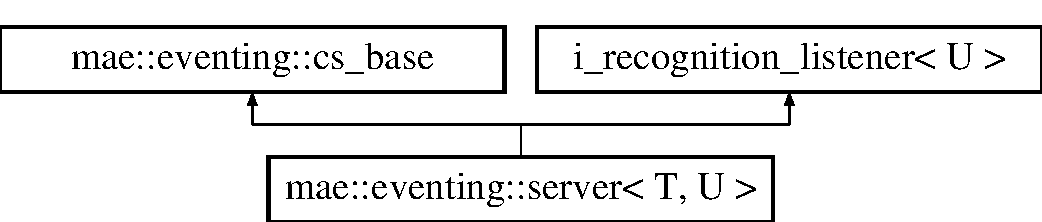
\includegraphics[height=2.000000cm]{classmae_1_1eventing_1_1server}
\end{center}
\end{figure}
\subsection*{Public Member Functions}
\begin{DoxyCompactItemize}
\item 
\hyperlink{classmae_1_1eventing_1_1server_aa160bd2b2d0398161b4218a0a74a651c}{server} (std\-::shared\-\_\-ptr$<$ \hyperlink{classmae_1_1eventing_1_1i__sequence__serializer}{i\-\_\-sequence\-\_\-serializer}$<$ U $>$ $>$ serializer, movement\-\_\-controller$<$ T, U $>$ $\ast$mov\-\_\-controller=nullptr, uint16\-\_\-t port=\hyperlink{classmae_1_1eventing_1_1cs__base_a5c068f50b548ec7299133976c00fa5a4}{cs\-\_\-base\-::get\-\_\-default\-\_\-port}(), std\-::string password=\char`\"{}\char`\"{}, bool debug=false)
\item 
virtual void \hyperlink{classmae_1_1eventing_1_1server_a94954a9ac22bbd73c36886815822fb8c}{notify\-\_\-clients} (long timestamp, std\-::vector$<$ std\-::shared\-\_\-ptr$<$ U $>$ $>$ sequences)
\item 
virtual std\-::list\\*
$<$ std\-::shared\-\_\-ptr\\*
$<$ \hyperlink{classmae_1_1eventing_1_1i__registration__manager}{i\-\_\-registration\-\_\-manager}$<$ U $>$ $>$ $>$ \hyperlink{classmae_1_1eventing_1_1server_acc7baf90eabaf3b7da1892d1ae95217e}{get\-\_\-registration\-\_\-managers} ()
\item 
virtual void \hyperlink{classmae_1_1eventing_1_1server_a7605c3953ad60a1ead4bc74c3085dcb5}{add\-\_\-registration\-\_\-manager} (std\-::shared\-\_\-ptr$<$ \hyperlink{classmae_1_1eventing_1_1i__registration__manager}{i\-\_\-registration\-\_\-manager}$<$ U $>$ $>$ manager)
\item 
virtual bool \hyperlink{classmae_1_1eventing_1_1server_a95e6e7b3e36fe6aaba85bbd5f4ca923f}{remove\-\_\-registration\-\_\-manager} (std\-::shared\-\_\-ptr$<$ \hyperlink{classmae_1_1eventing_1_1i__registration__manager}{i\-\_\-registration\-\_\-manager}$<$ U $>$ $>$ manager)
\item 
virtual void \hyperlink{classmae_1_1eventing_1_1server_ad2d13686ace9b9edac090834f82ef1b4}{register\-\_\-sequence} (std\-::shared\-\_\-ptr$<$ U $>$ sequence)
\item 
virtual void \hyperlink{classmae_1_1eventing_1_1server_adb20e7fbaa2413ea1897f2d0687c4e16}{on\-\_\-recognition} (long timestamp, std\-::vector$<$ std\-::shared\-\_\-ptr$<$ U $>$ $>$ sequences)
\item 
virtual void \hyperlink{classmae_1_1eventing_1_1server_a52c97fd5f391c6b26625201eb5d58c48}{on\-\_\-recognition} (long timestamp, std\-::vector$<$ std\-::string $>$ title)
\end{DoxyCompactItemize}
\subsection*{Protected Member Functions}
\begin{DoxyCompactItemize}
\item 
virtual void \hyperlink{classmae_1_1eventing_1_1server_a528106bf5539bc426074dd74aa601b4a}{handle\-\_\-initial\-\_\-message} (std\-::shared\-\_\-ptr$<$ boost\-::asio\-::ip\-::tcp\-::socket $>$ \hyperlink{classmae_1_1eventing_1_1client}{client}, std\-::string message, std\-::string server\-\_\-password)
\item 
virtual void \hyperlink{classmae_1_1eventing_1_1server_ab866e35c548b06b5dd4b0353fda29537}{handle\-\_\-further\-\_\-message} (std\-::shared\-\_\-ptr$<$ boost\-::asio\-::ip\-::tcp\-::socket $>$ \hyperlink{classmae_1_1eventing_1_1client}{client}, std\-::string message)
\item 
virtual std\-::string \hyperlink{classmae_1_1eventing_1_1server_a7d764a75a113c9dbe41d7cc21300ae4f}{create\-\_\-recognition\-\_\-message} (long timestamp, std\-::vector$<$ std\-::shared\-\_\-ptr$<$ U $>$ $>$ sequences, bool short\-\_\-message)
\item 
virtual void \hyperlink{classmae_1_1eventing_1_1server_a244c1e9b84052e3e745b39a8195550fc}{accept\-\_\-client} (std\-::shared\-\_\-ptr$<$ boost\-::asio\-::ip\-::tcp\-::socket $>$ connection, bool short\-\_\-message)
\item 
virtual void \hyperlink{classmae_1_1eventing_1_1server_a1835468f4fadde7ccbf888a2604f0845}{remove\-\_\-client} (std\-::shared\-\_\-ptr$<$ boost\-::asio\-::ip\-::tcp\-::socket $>$ connection)
\end{DoxyCompactItemize}
\subsection*{Additional Inherited Members}


\subsection{Constructor \& Destructor Documentation}
\hypertarget{classmae_1_1eventing_1_1server_aa160bd2b2d0398161b4218a0a74a651c}{\index{mae\-::eventing\-::server@{mae\-::eventing\-::server}!server@{server}}
\index{server@{server}!mae::eventing::server@{mae\-::eventing\-::server}}
\subsubsection[{server}]{\setlength{\rightskip}{0pt plus 5cm}template$<$typename T, typename U$>$ {\bf mae\-::eventing\-::server}$<$ T, U $>$\-::{\bf server} (
\begin{DoxyParamCaption}
\item[{std\-::shared\-\_\-ptr$<$ {\bf i\-\_\-sequence\-\_\-serializer}$<$ U $>$ $>$}]{serializer, }
\item[{movement\-\_\-controller$<$ T, U $>$ $\ast$}]{mov\-\_\-controller = {\ttfamily nullptr}, }
\item[{uint16\-\_\-t}]{port = {\ttfamily {\bf cs\-\_\-base\-::get\-\_\-default\-\_\-port}()}, }
\item[{std\-::string}]{password = {\ttfamily \char`\"{}\char`\"{}}, }
\item[{bool}]{debug = {\ttfamily false}}
\end{DoxyParamCaption}
)}}\label{classmae_1_1eventing_1_1server_aa160bd2b2d0398161b4218a0a74a651c}
Creates a new server based on boost sockets.


\begin{DoxyParams}{Parameters}
{\em serializer} & The serializer which is used to parse received sequences and serialize outgoing ones. \\
\hline
{\em mov\-\_\-controller} & The movement controller to which sequences are registered if any received from a client. \\
\hline
{\em port} & The port to be worked on. \\
\hline
{\em password} & The server password. \\
\hline
{\em debug} & True for debug output. \\
\hline
\end{DoxyParams}


\subsection{Member Function Documentation}
\hypertarget{classmae_1_1eventing_1_1server_a244c1e9b84052e3e745b39a8195550fc}{\index{mae\-::eventing\-::server@{mae\-::eventing\-::server}!accept\-\_\-client@{accept\-\_\-client}}
\index{accept\-\_\-client@{accept\-\_\-client}!mae::eventing::server@{mae\-::eventing\-::server}}
\subsubsection[{accept\-\_\-client}]{\setlength{\rightskip}{0pt plus 5cm}template$<$typename T , typename U $>$ void {\bf mae\-::eventing\-::server}$<$ T, U $>$\-::accept\-\_\-client (
\begin{DoxyParamCaption}
\item[{std\-::shared\-\_\-ptr$<$ boost\-::asio\-::ip\-::tcp\-::socket $>$}]{connection, }
\item[{bool}]{short\-\_\-message}
\end{DoxyParamCaption}
)\hspace{0.3cm}{\ttfamily [protected]}, {\ttfamily [virtual]}}}\label{classmae_1_1eventing_1_1server_a244c1e9b84052e3e745b39a8195550fc}
Accepts a client and registers the requested message format.


\begin{DoxyParams}{Parameters}
{\em connection} & The client. \\
\hline
{\em short\-\_\-message} & The message format. True for short messages. \\
\hline
\end{DoxyParams}
\hypertarget{classmae_1_1eventing_1_1server_a7605c3953ad60a1ead4bc74c3085dcb5}{\index{mae\-::eventing\-::server@{mae\-::eventing\-::server}!add\-\_\-registration\-\_\-manager@{add\-\_\-registration\-\_\-manager}}
\index{add\-\_\-registration\-\_\-manager@{add\-\_\-registration\-\_\-manager}!mae::eventing::server@{mae\-::eventing\-::server}}
\subsubsection[{add\-\_\-registration\-\_\-manager}]{\setlength{\rightskip}{0pt plus 5cm}template$<$typename T , typename U$>$ void {\bf mae\-::eventing\-::server}$<$ T, U $>$\-::add\-\_\-registration\-\_\-manager (
\begin{DoxyParamCaption}
\item[{std\-::shared\-\_\-ptr$<$ {\bf i\-\_\-registration\-\_\-manager}$<$ U $>$ $>$}]{manager}
\end{DoxyParamCaption}
)\hspace{0.3cm}{\ttfamily [virtual]}}}\label{classmae_1_1eventing_1_1server_a7605c3953ad60a1ead4bc74c3085dcb5}
Adds another registration manager to the server. The registered managers handle received sequences that are intended to be added to a movement controller.


\begin{DoxyParams}{Parameters}
{\em manager} & The manager. \\
\hline
\end{DoxyParams}
\hypertarget{classmae_1_1eventing_1_1server_a7d764a75a113c9dbe41d7cc21300ae4f}{\index{mae\-::eventing\-::server@{mae\-::eventing\-::server}!create\-\_\-recognition\-\_\-message@{create\-\_\-recognition\-\_\-message}}
\index{create\-\_\-recognition\-\_\-message@{create\-\_\-recognition\-\_\-message}!mae::eventing::server@{mae\-::eventing\-::server}}
\subsubsection[{create\-\_\-recognition\-\_\-message}]{\setlength{\rightskip}{0pt plus 5cm}template$<$typename T , typename U$>$ std\-::string {\bf mae\-::eventing\-::server}$<$ T, U $>$\-::create\-\_\-recognition\-\_\-message (
\begin{DoxyParamCaption}
\item[{long}]{timestamp, }
\item[{std\-::vector$<$ std\-::shared\-\_\-ptr$<$ U $>$ $>$}]{sequences, }
\item[{bool}]{short\-\_\-message}
\end{DoxyParamCaption}
)\hspace{0.3cm}{\ttfamily [protected]}, {\ttfamily [virtual]}}}\label{classmae_1_1eventing_1_1server_a7d764a75a113c9dbe41d7cc21300ae4f}
Creates a recognition message which informs the client on recognized sequences. This method is invoked for each client.


\begin{DoxyParams}{Parameters}
{\em timestamp} & The timestamp of the recognition event. \\
\hline
{\em sequences} & The recognized sequences. \\
\hline
{\em short\-\_\-message} & True if the message is intended to be short. \\
\hline
\end{DoxyParams}
\begin{DoxyReturn}{Returns}
The message string. 
\end{DoxyReturn}
\hypertarget{classmae_1_1eventing_1_1server_acc7baf90eabaf3b7da1892d1ae95217e}{\index{mae\-::eventing\-::server@{mae\-::eventing\-::server}!get\-\_\-registration\-\_\-managers@{get\-\_\-registration\-\_\-managers}}
\index{get\-\_\-registration\-\_\-managers@{get\-\_\-registration\-\_\-managers}!mae::eventing::server@{mae\-::eventing\-::server}}
\subsubsection[{get\-\_\-registration\-\_\-managers}]{\setlength{\rightskip}{0pt plus 5cm}template$<$typename T , typename U $>$ std\-::list$<$ std\-::shared\-\_\-ptr$<$ {\bf i\-\_\-registration\-\_\-manager}$<$ U $>$ $>$ $>$ {\bf mae\-::eventing\-::server}$<$ T, U $>$\-::get\-\_\-registration\-\_\-managers (
\begin{DoxyParamCaption}
{}
\end{DoxyParamCaption}
)\hspace{0.3cm}{\ttfamily [virtual]}}}\label{classmae_1_1eventing_1_1server_acc7baf90eabaf3b7da1892d1ae95217e}
Returns all registered registration managers.

\begin{DoxyReturn}{Returns}
The managers. 
\end{DoxyReturn}
\hypertarget{classmae_1_1eventing_1_1server_ab866e35c548b06b5dd4b0353fda29537}{\index{mae\-::eventing\-::server@{mae\-::eventing\-::server}!handle\-\_\-further\-\_\-message@{handle\-\_\-further\-\_\-message}}
\index{handle\-\_\-further\-\_\-message@{handle\-\_\-further\-\_\-message}!mae::eventing::server@{mae\-::eventing\-::server}}
\subsubsection[{handle\-\_\-further\-\_\-message}]{\setlength{\rightskip}{0pt plus 5cm}template$<$typename T , typename U $>$ void {\bf mae\-::eventing\-::server}$<$ T, U $>$\-::handle\-\_\-further\-\_\-message (
\begin{DoxyParamCaption}
\item[{std\-::shared\-\_\-ptr$<$ boost\-::asio\-::ip\-::tcp\-::socket $>$}]{client, }
\item[{std\-::string}]{message}
\end{DoxyParamCaption}
)\hspace{0.3cm}{\ttfamily [protected]}, {\ttfamily [virtual]}}}\label{classmae_1_1eventing_1_1server_ab866e35c548b06b5dd4b0353fda29537}
Handles any further message received from the client. This message is the sequence registration message and if the sequence is parsed the register\-\_\-sequence method is invoked.


\begin{DoxyParams}{Parameters}
{\em client} & The client. \\
\hline
{\em message} & The received message. \\
\hline
\end{DoxyParams}
\hypertarget{classmae_1_1eventing_1_1server_a528106bf5539bc426074dd74aa601b4a}{\index{mae\-::eventing\-::server@{mae\-::eventing\-::server}!handle\-\_\-initial\-\_\-message@{handle\-\_\-initial\-\_\-message}}
\index{handle\-\_\-initial\-\_\-message@{handle\-\_\-initial\-\_\-message}!mae::eventing::server@{mae\-::eventing\-::server}}
\subsubsection[{handle\-\_\-initial\-\_\-message}]{\setlength{\rightskip}{0pt plus 5cm}template$<$typename T , typename U $>$ void {\bf mae\-::eventing\-::server}$<$ T, U $>$\-::handle\-\_\-initial\-\_\-message (
\begin{DoxyParamCaption}
\item[{std\-::shared\-\_\-ptr$<$ boost\-::asio\-::ip\-::tcp\-::socket $>$}]{client, }
\item[{std\-::string}]{message, }
\item[{std\-::string}]{server\-\_\-password}
\end{DoxyParamCaption}
)\hspace{0.3cm}{\ttfamily [protected]}, {\ttfamily [virtual]}}}\label{classmae_1_1eventing_1_1server_a528106bf5539bc426074dd74aa601b4a}
Handles the initial message received from a newly connected client. If password is fine, the client is accepted and the accept\-\_\-client method is invoked.


\begin{DoxyParams}{Parameters}
{\em client} & The newly connected client. \\
\hline
{\em message} & The received message. \\
\hline
{\em server\-\_\-password} & The password for the server. \\
\hline
\end{DoxyParams}
\hypertarget{classmae_1_1eventing_1_1server_a94954a9ac22bbd73c36886815822fb8c}{\index{mae\-::eventing\-::server@{mae\-::eventing\-::server}!notify\-\_\-clients@{notify\-\_\-clients}}
\index{notify\-\_\-clients@{notify\-\_\-clients}!mae::eventing::server@{mae\-::eventing\-::server}}
\subsubsection[{notify\-\_\-clients}]{\setlength{\rightskip}{0pt plus 5cm}template$<$typename T , typename U$>$ void {\bf mae\-::eventing\-::server}$<$ T, U $>$\-::notify\-\_\-clients (
\begin{DoxyParamCaption}
\item[{long}]{timestamp, }
\item[{std\-::vector$<$ std\-::shared\-\_\-ptr$<$ U $>$ $>$}]{sequences}
\end{DoxyParamCaption}
)\hspace{0.3cm}{\ttfamily [virtual]}}}\label{classmae_1_1eventing_1_1server_a94954a9ac22bbd73c36886815822fb8c}
Notifies all connected clients on recognized sequences.


\begin{DoxyParams}{Parameters}
{\em timestamp} & The timestamp. \\
\hline
{\em sequences} & The recognized sequences. \\
\hline
\end{DoxyParams}
\hypertarget{classmae_1_1eventing_1_1server_adb20e7fbaa2413ea1897f2d0687c4e16}{\index{mae\-::eventing\-::server@{mae\-::eventing\-::server}!on\-\_\-recognition@{on\-\_\-recognition}}
\index{on\-\_\-recognition@{on\-\_\-recognition}!mae::eventing::server@{mae\-::eventing\-::server}}
\subsubsection[{on\-\_\-recognition}]{\setlength{\rightskip}{0pt plus 5cm}template$<$typename T , typename U$>$ void {\bf mae\-::eventing\-::server}$<$ T, U $>$\-::on\-\_\-recognition (
\begin{DoxyParamCaption}
\item[{long}]{timestamp, }
\item[{std\-::vector$<$ std\-::shared\-\_\-ptr$<$ U $>$ $>$}]{sequences}
\end{DoxyParamCaption}
)\hspace{0.3cm}{\ttfamily [virtual]}}}\label{classmae_1_1eventing_1_1server_adb20e7fbaa2413ea1897f2d0687c4e16}
Is invoked each time sequences were recognized.


\begin{DoxyParams}{Parameters}
{\em timestamp} & The associated timestamp. \\
\hline
{\em sequences} & The recognized sequences. \\
\hline
\end{DoxyParams}
\hypertarget{classmae_1_1eventing_1_1server_a52c97fd5f391c6b26625201eb5d58c48}{\index{mae\-::eventing\-::server@{mae\-::eventing\-::server}!on\-\_\-recognition@{on\-\_\-recognition}}
\index{on\-\_\-recognition@{on\-\_\-recognition}!mae::eventing::server@{mae\-::eventing\-::server}}
\subsubsection[{on\-\_\-recognition}]{\setlength{\rightskip}{0pt plus 5cm}template$<$typename T , typename U$>$ void {\bf mae\-::eventing\-::server}$<$ T, U $>$\-::on\-\_\-recognition (
\begin{DoxyParamCaption}
\item[{long}]{timestamp, }
\item[{std\-::vector$<$ std\-::string $>$}]{title}
\end{DoxyParamCaption}
)\hspace{0.3cm}{\ttfamily [virtual]}}}\label{classmae_1_1eventing_1_1server_a52c97fd5f391c6b26625201eb5d58c48}
Is invoked each time sequences were recognized and only titles of the sequences are present.


\begin{DoxyParams}{Parameters}
{\em timestamp} & The associated timestamp. \\
\hline
{\em sequences} & The recognized sequences. \\
\hline
\end{DoxyParams}
\hypertarget{classmae_1_1eventing_1_1server_ad2d13686ace9b9edac090834f82ef1b4}{\index{mae\-::eventing\-::server@{mae\-::eventing\-::server}!register\-\_\-sequence@{register\-\_\-sequence}}
\index{register\-\_\-sequence@{register\-\_\-sequence}!mae::eventing::server@{mae\-::eventing\-::server}}
\subsubsection[{register\-\_\-sequence}]{\setlength{\rightskip}{0pt plus 5cm}template$<$typename T , typename U$>$ void {\bf mae\-::eventing\-::server}$<$ T, U $>$\-::register\-\_\-sequence (
\begin{DoxyParamCaption}
\item[{std\-::shared\-\_\-ptr$<$ U $>$}]{sequence}
\end{DoxyParamCaption}
)\hspace{0.3cm}{\ttfamily [virtual]}}}\label{classmae_1_1eventing_1_1server_ad2d13686ace9b9edac090834f82ef1b4}
Registers a sequence to the connected controller if any.


\begin{DoxyParams}{Parameters}
{\em sequence} & The sequence to be registered. \\
\hline
\end{DoxyParams}
\hypertarget{classmae_1_1eventing_1_1server_a1835468f4fadde7ccbf888a2604f0845}{\index{mae\-::eventing\-::server@{mae\-::eventing\-::server}!remove\-\_\-client@{remove\-\_\-client}}
\index{remove\-\_\-client@{remove\-\_\-client}!mae::eventing::server@{mae\-::eventing\-::server}}
\subsubsection[{remove\-\_\-client}]{\setlength{\rightskip}{0pt plus 5cm}template$<$typename T , typename U $>$ void {\bf mae\-::eventing\-::server}$<$ T, U $>$\-::remove\-\_\-client (
\begin{DoxyParamCaption}
\item[{std\-::shared\-\_\-ptr$<$ boost\-::asio\-::ip\-::tcp\-::socket $>$}]{connection}
\end{DoxyParamCaption}
)\hspace{0.3cm}{\ttfamily [protected]}, {\ttfamily [virtual]}}}\label{classmae_1_1eventing_1_1server_a1835468f4fadde7ccbf888a2604f0845}
Removes the client from the connection list and closes the connection to the client.


\begin{DoxyParams}{Parameters}
{\em connection} & The client. \\
\hline
\end{DoxyParams}
\hypertarget{classmae_1_1eventing_1_1server_a95e6e7b3e36fe6aaba85bbd5f4ca923f}{\index{mae\-::eventing\-::server@{mae\-::eventing\-::server}!remove\-\_\-registration\-\_\-manager@{remove\-\_\-registration\-\_\-manager}}
\index{remove\-\_\-registration\-\_\-manager@{remove\-\_\-registration\-\_\-manager}!mae::eventing::server@{mae\-::eventing\-::server}}
\subsubsection[{remove\-\_\-registration\-\_\-manager}]{\setlength{\rightskip}{0pt plus 5cm}template$<$typename T , typename U$>$ bool {\bf mae\-::eventing\-::server}$<$ T, U $>$\-::remove\-\_\-registration\-\_\-manager (
\begin{DoxyParamCaption}
\item[{std\-::shared\-\_\-ptr$<$ {\bf i\-\_\-registration\-\_\-manager}$<$ U $>$ $>$}]{manager}
\end{DoxyParamCaption}
)\hspace{0.3cm}{\ttfamily [virtual]}}}\label{classmae_1_1eventing_1_1server_a95e6e7b3e36fe6aaba85bbd5f4ca923f}
Removes a registration manager from the controller.


\begin{DoxyParams}{Parameters}
{\em manager} & The manager. \\
\hline
\end{DoxyParams}
\begin{DoxyReturn}{Returns}
True if successful. 
\end{DoxyReturn}


The documentation for this class was generated from the following file\-:\begin{DoxyCompactItemize}
\item 
src/mae/eventing/server.\-hpp\end{DoxyCompactItemize}

%--- End generated contents ---

% Index
\newpage
\phantomsection
\addcontentsline{toc}{chapter}{Index}
\printindex

\end{document}
